\documentclass[a4paper,12pt,oneside]{article}

\usepackage[a4paper]{geometry}
\usepackage{amssymb,amsmath}
\usepackage{amsthm}
\usepackage[utf8]{inputenc}
\usepackage{enumerate}
\usepackage{color}
\usepackage{graphicx}
\usepackage[estonian]{babel}
\usepackage[usenames,dvipsnames]{xcolor}
\usepackage{float}
\usepackage{cite}
\usepackage{etoolbox}
\usepackage{theoremref}
\usepackage[hidelinks]{hyperref}
\usepackage{tikz}
\usepackage{framed}
\usepackage[framemethod=tikz]{mdframed}
\usepackage{diagbox}
\usepackage{pifont}
\usepackage{colortbl}
\usepackage{minted}
\usepackage{caption}
\usepackage[parfill]{parskip}
\usepackage{verbatim}
\usepackage{tocbibind}
\usepackage[toc,titletoc]{appendix}
\usepackage{afterpage}

\renewcommand{\appendixtocname}{Lisad}
\renewcommand{\appendixtocname}{Lisad}

\renewcommand{\setthesubsection}{\Alph{subsection}}

\DeclareCaptionType{mytype}[Typename][List of mytype]

\newenvironment{customFloatWrap}{}{}

\newfloat{Programm}{thp}{prog}
% replace minted@colorbg definition
% also, remove minted@bgbox definition
% or replace all usages with mdframed directly
\renewenvironment{minted@colorbg}[1]{%
 % may want to leave out "style=default" to allow users some control
 % instead set linewidth=0 as the default, and leave only bgcolor setting
 \begin{mdframed}[style=default,linewidth=0,backgroundcolor=#1]}
 {\end{mdframed}}

\renewcommand\thefootnote{\ding{\numexpr171+\value{footnote}}}

\renewcommand{\thempfootnote}{$\mathsection$}%  


\allowdisplaybreaks
\makeatletter
\patchcmd{\HyField@FlagsRadioButton}{\HyField@SetFlag{Ff}{Radio}}{}{}{}
\makeatother
\def\DefaultOptionsofRadio{print}



\definecolor{background_example}{HTML}{EDEDED}
\definecolor{table_red}{HTML}{c8c8c8}
\definecolor{table_blue}{HTML}{d2d2d2}
%E0DCDE


\newcommand{\nocontentsline}[3]{}
\newcommand{\tocless}[2]{\bgroup\let\addcontentsline=\nocontentsline#1{#2}\egroup}

%\setlength\parindent{0pt}
\newenvironment{tightcenter}{%
  \setlength\topsep{0pt}
  \setlength\parskip{0pt}
  \begin{center}
}{%
  \end{center}
}
\newsavebox{\thisOne}
\newenvironment{meeldetuletus}{
	\begin{lrbox}{\thisOne}
		\begin{minipage}{0.95\textwidth} \vspace{0.25em} {\scriptsize \textsc{meeldetuletuseks}} \linebreak \vspace{-0.5em}
} 
{  
 \end{minipage}\end{lrbox}{
 		
 			\begin{mdframed}[tikzsetting={draw=black,dashed,line width=0.5pt, dash pattern = on 10pt off 3pt},%
 			linecolor=background_example,backgroundcolor=background_example,outerlinewidth=1pt]
			
 			\usebox{\thisOne}
 			\end{mdframed}
 		
 		
 	}
}
\newsavebox{\boxTwo}
\newenvironment{naide}{
    \begin{lrbox}{\boxTwo}
        \begin{minipage}{\textwidth}
    }
    {\end{minipage}\end{lrbox}
    	\colorbox{background_example}{\usebox{\boxTwo}}
    }

\author{Vootele Rõtov}
\title{Valikvastustega küsimustike reliaabluse hindamine}

\newcounter{lemma}[section]
\numberwithin{equation}{section}
\theoremstyle{definition}
\newtheorem*{elementaarsyndmus}{Definitsioon}
\newtheorem*{toenaosus}{Definitsioon}
\newtheorem*{juhuslik_suurus}{Definitsioon}
\newtheorem*{jaotus}{Definitsioon}
\newtheorem*{keskvaartus}{Definitsioon}
\newtheorem*{dispersioon}{Definitsioon}
\newtheorem{keskvaartus_konstant}[equation]{Lause}
\newtheorem{dispersioon_konstant}[equation]{Lause}
\newtheorem*{kovariatsioon}{Definitsioon}
\newtheorem*{korrelatsioon}{Definitsioon}
\newtheorem{summa_dispersioon}[equation]{Lause}
\newtheorem{summa_kovariatsioon}[equation]{Lause}
\newtheorem*{mittenegatiivselt_maaratud}{Definitsioon}
\newtheorem{konstant_kovariatsioon}[equation]{Lause}
\newtheorem{lambda_1}[lemma]{Lemma}
\newtheorem{ii_times_jj}[lemma]{Lemma}
\newtheorem{helper_2}[lemma]{Lemma}
\newtheorem{lambda_2}[lemma]{Lemma}
\newtheorem{lambda_3}[lemma]{Lemma}
\newtheorem{lambda_4}[lemma]{Lemma}
\newtheorem{glb}[lemma]{Lemma}

\begin{document}



\makeatletter
\begin{titlepage}
\begin{center}

{\large TARTU ÜLIKOOL}\\[0.3cm]
{\large MATEMAATIKA-INFORMAATIKATEADUSKOND}\\[0.3cm]
{\large Matemaatika instituut}\\[0.3cm]
{\large Matemaatika eriala} %\\[3cm]

\vfill
{\large \@author}\\[0.3cm]
{\huge \textbf{\@title}}\\[0.3cm]
{\large Bakalaureusetöö (6 EAP)} %\\[3cm]

\vfill

\begin{flushright}
{\large Juhendaja: Margus Niitsoo}
\end{flushright}
 

\vfill

{\large TARTU \the\year}

\end{center}
\end{titlepage}
\makeatother

\pagebreak

\makeatletter
\tocless{\subsection*{\@title}}

\tocless{\subsubsection*{\@author}}

\tocless{\subsubsection*{Lühikokkuvõte}}

\makeatother

Käesolevas bakalaureusetöös vaadeldakse erinevaid võimalusi valikvastustega kü\-si\-mus\-tike reliaabluse hindamiseks küsimustiku ühekordse läbiviimise põhjal. 

Töö käigus antakse lugejale vajaminevad taustteadmised valikvastustega küsimus\-tike ning nende karakteristikute kohta, defineeritakse reliaablus klassikalise testiteooria raamistikus ja antakse vajalik matemaatiline baas reliaabluse hinnangute tuletamiseks. Seejärel tuletatakse viis reliaabluse hinnangut, hinnatakse nende \linebreak kasutatavust praktikas ja tutvustatakse autori loodud programmiteeki, mis sisaldab programme tuletatud hinnangute leidmiseks küsimustiku läbiviimisel saadud \linebreak andmete põhjal. Töö viimases osas tutvustab autor üht võimalikku viisi küsimustike arvulise tõlgenduse parandamiseks.

Töö annab eesti keelse ülevaate klassikalise testiteooria alustest matemaatilisest vaatepunktist lähtudes, ning tutvustab praktikule erinevaid võimalusi testi reliaabluse hindamiseks, sealjuures tutvustatake meetodeid, millest osad annavad täpsemaid tulemusi, kui hetkel enamlevinud meetodid. 


\textsc{võtmesõnad:} psühhomeetria, klassikaline testiteooria,  valikvastustega kü\-si\-mus\-tikud, reliaablus, reliaabluse hindamine,  Cronbachi alfa, Guttmani lambdad, glb. 

\pagebreak

\makeatletter
\tocless{\subsection*{On the Reliability of Likert Scale Questionnaires}}

\tocless{\subsubsection*{\@author}}

\tocless{\subsubsection*{Abstract}}



\makeatother

This bachelor's thesis gives an overview of different possibilities of estimating the reliability of Likert scale questionnaires based on a single admission.

The thesis contains a short overview of the necessary background information about Likert scales and their characteristics, definition of reliability in the context of the Classical Test Theory and mathematical basis for deriving estimations of reliability. Also, five estimates are derived and their usability in practise is discussed. Afterwards, the author gives a short overview of a programming library that implements methods for finding derived estimates based on data gathered with the questionnaire. Finally, the author proposes an approach for improving the quantitative interpretation of a questionnaire.

The thesis gives an overview of the foundations of the Classical Test Theory in Estonian from a mathematical viewpoint and introduces different possibilities for estimating the reliability of a questionnaire, some of which give more exact estimates than the ones in widespread use today.

\textsc{keywords:}  psychometrics, classical test theory, Likert scale questionnaires, reliability, estimating reliability, Cronbach's alfa, Guttman's lambdas, glb.

\pagebreak


\tableofcontents

\pagebreak

\section*{Sissejuhatus}
\addcontentsline{toc}{section}{Sissejuhatus}

Käesolev bakalaureusetöö on ajendatud psühholoogide probleemist -- kuidas \linebreak hinnata nende töövaldkonnas tihti kasutatavate valikvastustega küsimustike usaldusväärsust. {\color{red} midagi ka selle kohta, et testi reliaablust tõsta}

Sellest lähtuvalt on töö peamiseks eesmärgiks uurida valikvastustega küsimustike hindamiseks lihtsasti kasutatavaid kvantitatiivseid meetodeid. Lisaks sellele loodab autor pakkuda eestikeelset ülevaadet ühest valikvastustega testidega seotud matemaatiliselt raamistikust. Olemasolevad käsitlused on pigem praktilised abivahendid psühholoogidele. 
{\color{red}viimasest osast}

Töö esimeses osas esitame vajaliku taustinfo, definitsioonid ja probleemipüstituse. Seejärel ehitame üles meile vajamineva osa probleemi vaatlemiseks sobivast matemaatilisest teooriast -- defineerime testi usaldusväärsuse ning rajame vundamendi selle hindamiseks. Järgnevalt tuletame mõningad erinevad usaldusväärsuse hinnangud. Seejärel tutvustame autori loodud programmiteeki, mis sisaldab eelnevalt tutvustatud hinnangute implementatsioone. Töö viimases osas pakub autor välja alternatiivse lähenemise küsimustiku vastuste arvulisele tõlgendamisele.

Autori eesmärgiks on, et antud tekst oleks lihtsasti järgitav keskmisele bakalaureuseõppe läbinud matemaatikatudengile -- meeldetuletuseks on valdkonnaspetsiifilised matemaatilised definitsioonid ja tulemused töö käigus jooksvalt ära \linebreak toodud. 

Lisaks loodab autor, et loodud programmiteek pakkub huvi ka psühholoogidele. 

Autor soovib tänada Margus Niitsood konstruktiivse juhendamise eest ning Timo Aavat ja Kadi Kähär-Petersoni abi eest käesolevas bakalaureusetöös kasutatud artiklite kättesaadavaks tegemisel.    






\pagebreak



\section{Taustinfo ja probleemipüstitus}

Järgnevalt anname probleemi mõtestamiseks vajalikud taustateadmised ning pea\-tüki lõpetuseks püstitame käesoleva töö keskse probleemi. {\color{red} probleemid}

\subsection{Küsimustik, küsimus ja Likerti skaala}

Käesolev uurimus tegeleb k\"usimustikega (\textit{Likert scale}),  milles soovitakse hinnan\-guid teatud arvule küsimustele (\textit{Likert item}) $n$-pallisel Likerti skaalal \cite{Edmondson}, kus $n$ jääb enamasi kahe ja kümne vahele.  Käsitleme Likerti skaalasid, mis on sümmeetrilised, see tähendab, et positiivsete ja negatiivsete vastusevariantide arv on sama. Näiteks:\footnote{Terviklike k\"usimustike näited on esitatud lisades, \hyperref[likert1]{joonisel \ref*{likert1}} ja \hyperref[likert2]{\ref*{likert2}}}

\vspace{10pt}

\begin{figure}[H]


\colorbox{background_example}{\parbox{\textwidth}{

\vspace{1mm}

Käesoleva bakalaureusetöö \"ulesehitus on loogiline.

\vspace{5pt}

\begin{Form}
\def\DefaultWidthofChoiceMenu{12pt}%


\small{
	\CheckBox[bordercolor = gray,name=optionE]{\mbox{}} Ei nõustu 
	\CheckBox[bordercolor = gray,name=optionD]{\mbox{}} Ei nõustu osaliselt
	\CheckBox[bordercolor = gray,name=optionC]{\mbox{}} Nii ja naa
	\CheckBox[bordercolor = gray,name=optionC]{\mbox{}}  Nõustun osaliselt
	\CheckBox[checked,bordercolor = gray,name=optionC]{\mbox{}} Nõustun
}


\end{Form}}}
\caption{Näide väitest, millele palutakse hinnangut Likerti skaalal}
\label{likert_question}
\end{figure}

\subsection{Likerti skaala tõlgendamine intervallskaalana}

Likerti skaala tõlgendamisel intervallksaalana on välja kujunenud tava seada valikvastustele vastavusse järjestatud täisarvud, kusjuures mida positiivsem on vastuse variant, seda suurem on temale vastavusse seatud arv. Reeglina kasutatakse kas arve alates ühest kuni valikvastuste arvuni või valitakse välja täisarvud nii, et neutraalsele vastusevariandile vastab null.

\begin{figure}[H]

\colorbox{background_example}{\parbox{\textwidth}{

\vspace{1mm}

Käesoleva bakalaureusetöö \"ulesehitus on loogiline.

\vspace{5pt}

\begin{tikzpicture}
\node at (0,0) {};
\draw[very thick, ->] (0.625em,0em) -- (0.625em,1.5em) node[label=above: -2] {};
\draw[very thick, ->] (6.375em,0em) -- (6.375em,1.5em) node[label=above: -1] {};
\draw[very thick, ->] (15.75em,0em) -- (15.75em,1.5em) node[label=above: 0] {};
\draw[very thick, ->] (21.625em,0em) -- (21.625em,1.5em) node[label=above: 1] {};
\draw[very thick, ->] (30.5em,0em) -- (30.5em,1.5em) node[label=above: 2] {};
\end{tikzpicture}

\begin{Form}
\def\DefaultWidthofChoiceMenu{12pt}%
\small{
\CheckBox[bordercolor = gray,name=optionE1]{\mbox{}} Ei nõustu 
\CheckBox[bordercolor = gray,name=optionD1]{\mbox{}} Ei nõustu osaliselt
\CheckBox[bordercolor = gray,name=optionC1]{\mbox{}} Nii ja naa
\CheckBox[checked,bordercolor = gray,name=optionC1]{\mbox{}}  Nõustun osaliselt
\CheckBox[bordercolor = gray,name=optionC1]{\mbox{}} Nõustun
}
\end{Form}



\begin{tikzpicture}
\node at (0,0) {};
\draw[very thick, ->] (0.625em,0em) -- (0.625em,-1.5em) node[label=below: 1] {};
\draw[very thick, ->] (6.375em,0em) -- (6.375em,-1.5em) node[label=below: 2] {};
\draw[very thick, ->] (15.75em,0em) -- (15.75em,-1.5em) node[label=below: 3] {};
\draw[very thick, ->] (21.625em,0em) -- (21.625em,-1.5em) node[label=below: 4] {};
\draw[very thick, ->] (30.5em,0em) -- (30.5em,-1.5em) node[label=below: 5] {};
\end{tikzpicture}}}
\caption{Näide kahest levinumast Likerti skaala tõlgendusest invtervallskaalana }
\label{likert_question}
\end{figure}

Lugejal võib tekkida õigustatud k\"usimus, kuidas põhjendab autor Likerti skaala käsitlemist intervallskaalana, kui Likerti skaala on olemuselt järjestikskaala ning selle tõlgendamine intervallskaalana on vastuoluline küsimus, näiteks \cite{Jamieson2004}. Siinkohal tõdeme, et Likerti skaala tõlgendamine intervallksaalana on praktikas piisavalt levinud, et selle valdkonna uurimine oleks õigustatud, olenemata selle teoreetilisest põhjendatusest.  Siinkohal väärib autori silmis esile toomist kriitikute \"uks levinumaid argumente: "`hea"' ja "`väga hea"'  keskmine ei ole  loomulikul viisil tõlgendatav kui "`hea + pool"' ehk pole põhjust eeldada, et kõikide küsimuste omavaheline kaugus on mingil põhjusel võrdne. 



\subsection{Küsimustiku valiidsus}

Küsimustiku \textbf{valiidsus} on küsimustiku karakteristik, mis iseloomustab küsimustiku võimet mõõta seda, mida see kujundati mõõtma. Enamikes käsitlustes vaadeldakse valiidsust kui väärtust intervallskaalal nulli ja ühe vahel.

Näitena olgu meil küsimustikuks kaal, mille näitu vaatleme kui küsimustiku tulemust kaalutava isiku puhul. Kaal, mis näitab 75 kilo kaaluva inimese kaaluks 74,5 kilo, omab kõrgemat valiidsust, kui kaal, mis sama inimese puhul näitab kaaluks 65 kilo.   


Küsimustiku valiidsuse mõtestamisel võime kasutada analoogiat täpsuslaskmisega. Kui vaatleme küsimustikke kui laskureid, siis tähendab see, et laskuri $A$ valiidus on kõrgem kui laskuri $B$ oma seda,et tema tabamused asuvad märklaua keskkohale lähemal. Olukorda illustreerib järgnev joonis:

\begin{figure}[H]
\begin{naide}
\begin{tikzpicture}
 \path[use as bounding box] (-6em,7.5em) rectangle (30em,-8em);
\filldraw[fill=red!80, draw=red!80] (5em,0) circle [radius=5.5em]; 
\filldraw[fill=white!80, draw=white!80] (5em,0) circle [radius=5em];
\filldraw[fill=red!80, draw=red!80] (5em,0) circle [radius=4.5em]; 
\filldraw[fill=white!80, draw=white!80] (5em,0) circle [radius=4em];
\filldraw[fill=red!80, draw=red!80] (5em,0) circle [radius=3.5em]; 
\filldraw[fill=white!80, draw=white!80] (5em,0) circle [radius=3em];
\filldraw[fill=red!80, draw=red!80] (5em,0) circle [radius=2.5em]; 
\filldraw[fill=white!80, draw=white!80] (5em,0) circle [radius=2em];
\filldraw[fill=red!80, draw=red!80] (5em,0) circle [radius=1.5em]; 
\filldraw[fill=white!80, draw=white!80] (5em,0) circle [radius=1em];
\filldraw[fill=red!80, draw=red!80] (5em,0) circle [radius=0.5em]; 


\filldraw[fill=red!80, draw=red!80] (20em,0) circle [radius=5.5em]; 
\filldraw[fill=white!80, draw=white!80] (20em,0) circle [radius=5em];
\filldraw[fill=red!80, draw=red!80] (20em,0) circle [radius=4.5em]; 
\filldraw[fill=white!80, draw=white!80] (20em,0) circle [radius=4em];
\filldraw[fill=red!80, draw=red!80] (20em,0) circle [radius=3.5em]; 
\filldraw[fill=white!80, draw=white!80] (20em,0) circle [radius=3em];
\filldraw[fill=red!80, draw=red!80] (20em,0) circle [radius=2.5em]; 
\filldraw[fill=white!80, draw=white!80] (20em,0) circle [radius=2em];
\filldraw[fill=red!80, draw=red!80] (20em,0) circle [radius=1.5em]; 
\filldraw[fill=white!80, draw=white!80] (20em,0) circle [radius=1em];
\filldraw[fill=red!80, draw=red!80] (20em,0) circle [radius=0.5em]; 

\foreach \x/\y in {5/0.75, 3.8/-0.45, 3.5/0, 5/0, 3.75/0.75, 4/1.25}
	\filldraw[fill=black, draw=black] (\x em,\y em) circle [radius=0.2em];

\foreach \x/\y in {17/0.75, 15.8/-0.45, 15.5/0, 17/0, 15.75/0.75, 16/1.25}
	\filldraw[fill=black, draw=black] (\x em,\y em) circle [radius=0.2em];

\node[label=below: A] at (5em,-6em) {};

\node[label=below: B] at (20em,-6em) {};



\end{tikzpicture}
\end{naide}
\caption{Kahe küsimustiku valiidsuse võrdlus}
\end{figure}


Arusaadavatel põhjustel on testi valiidsus äärmiselt oluline ning psühholoogiliste testide valiidsuse hindamine on olnud üks psühhomeetria põhilistest uurimisobjektidest. Sellega seoses on tehtud palju tööd  ka valiidsuse definitsiooni täpsemaks muutmisega, võrreldes selle paragrahvi alguses antud väga intuitiivse definitsiooniga. Kuna valiidsus on käesoleva töö raames vajalik vaid taustinfona probleemi mõtestamiseks, tundub antud lihtne definitsioon aga sobivaim. 

\subsection{Küsimustiku reliaablus}

Küsimustiku \textbf{reliaablus} on küsimustiku karakteristik, mis kirjeldab, kui järje\-pidevad on subjekti erinevad mõõtmised sama küsimustikuga. Nii nagu valiidsus, on ka reliaablus reeglina määratud intervallskaalal nulli ja ühe vahel. 

Näiteks kaal, mis näitab igal kaalumisel 75 kilo kaaluva inimese kaaluks 74,5 kilo, omab kõrgemat reliaablust, kui kaal, mis näitab juhuslikult kas 74,5 kilo või 75,5 kilo. 

Ka küsimustiku reliaabluse mõtestamisel saame kasutada analoogiat täpsus\-lask\-misega. Sellisel juhul tähendab see, et laskuri $A$ reliaablus on suurem kui laskuri $B$ oma seda, et laskuri $A$ tabamused asuvad teineteisele lähemal, kui laskuri $B$ tabamused. Olukorda illustreerib järgnev joonis:

\begin{figure}[H]
\begin{naide}
\begin{tikzpicture}
 \path[use as bounding box] (-6em,7.5em) rectangle (30em,-8em);
\filldraw[fill=red!80, draw=red!80] (5em,0) circle [radius=5.5em]; 
\filldraw[fill=white!80, draw=white!80] (5em,0) circle [radius=5em];
\filldraw[fill=red!80, draw=red!80] (5em,0) circle [radius=4.5em]; 
\filldraw[fill=white!80, draw=white!80] (5em,0) circle [radius=4em];
\filldraw[fill=red!80, draw=red!80] (5em,0) circle [radius=3.5em]; 
\filldraw[fill=white!80, draw=white!80] (5em,0) circle [radius=3em];
\filldraw[fill=red!80, draw=red!80] (5em,0) circle [radius=2.5em]; 
\filldraw[fill=white!80, draw=white!80] (5em,0) circle [radius=2em];
\filldraw[fill=red!80, draw=red!80] (5em,0) circle [radius=1.5em]; 
\filldraw[fill=white!80, draw=white!80] (5em,0) circle [radius=1em];
\filldraw[fill=red!80, draw=red!80] (5em,0) circle [radius=0.5em]; 


\filldraw[fill=red!80, draw=red!80] (20em,0) circle [radius=5.5em]; 
\filldraw[fill=white!80, draw=white!80] (20em,0) circle [radius=5em];
\filldraw[fill=red!80, draw=red!80] (20em,0) circle [radius=4.5em]; 
\filldraw[fill=white!80, draw=white!80] (20em,0) circle [radius=4em];
\filldraw[fill=red!80, draw=red!80] (20em,0) circle [radius=3.5em]; 
\filldraw[fill=white!80, draw=white!80] (20em,0) circle [radius=3em];
\filldraw[fill=red!80, draw=red!80] (20em,0) circle [radius=2.5em]; 
\filldraw[fill=white!80, draw=white!80] (20em,0) circle [radius=2em];
\filldraw[fill=red!80, draw=red!80] (20em,0) circle [radius=1.5em]; 
\filldraw[fill=white!80, draw=white!80] (20em,0) circle [radius=1em];
\filldraw[fill=red!80, draw=red!80] (20em,0) circle [radius=0.5em]; 

\foreach \x/\y in {6/4, 5.5/4.4, 6.4/3.5, 5.7/3.6, 6.7/4, 6.5/4.5}
	\filldraw[fill=black, draw=black] (\x em,\y em) circle [radius=0.2em];

\foreach \x/\y in {18/4, 17/3, 18/2, 19/4, 18.75/1.25, 21/2.25}
	\filldraw[fill=black, draw=black] (\x em,\y em) circle [radius=0.2em];

\node[label=below: A] at (5em,-6em) {};

\node[label=below: B] at (20em,-6em) {};


\end{tikzpicture}
\end{naide}
\caption{Kahe küsimustiku reliaabluse võrdlus}
\end{figure}

Paneme tähele, et kõrgem reliaablus ei tähenda tingimata seda, et testi valiidsus on suurem.

Reliaabluse täpsema, matemaatilise definitsiooni anname edaspidi. 

\subsection{Valiidsuse ja reliaabluse suhe}

Valiidsuse ja reliaabluse suhestamisel kerkib kiiresti üles loomulik küsimus -- kas test võib olla samaaegselt suure valiidsuse ja väikse reliaablusega? Eelpool antud definitsioonid jätavad selle küsimuse lahtiseks. Vaatleme järgmist olukorda:

\begin{figure}[H]
\colorbox{background_example}{\parbox{\textwidth}{
\begin{tikzpicture}
  \draw (0,0) -- (35em,0);
  \foreach \x/\xtext in {2.5/74,10/\text{74,5},17.5/75,25/\text{75,5},32.5/76}
  	\draw (\x em,0.75em) -- (\x em,-0.75em) node [anchor=north] {$\xtext$};
  \filldraw[fill=red!60,draw=red!80!black] (17.5em,0) circle [radius = 0.6em];
  \foreach \y in {2.5,17.5,32.5}
  	\filldraw[fill=green!75,draw=green!30!black] (\y em, 0) circle [radius = 0.4em];
  \filldraw[fill=blue!100,draw=blue!80] (10em,0) circle [radius = 0.5em];
  \filldraw[fill=blue!60,draw=blue!70] (10em,0) circle [radius = 0.4em];
  \filldraw[fill=blue!20,draw=blue!60] (10em,0) circle [radius = 0.3em];
  \filldraw[fill=green!75,draw=green!30!black] (1.5 em, -3em) circle [radius = 0.4em];
  \node[label=right:  Kaalu $1$ tulemused] at (1.5 em, -3em) {};
  \filldraw[fill=blue!60,draw=blue!70!black] (15em,-3em) circle [radius = 0.4em];
  \node[label=right:  Kaalu $2$ tulemused] at (15 em, -3em) {};
  \filldraw[fill=red!60,draw=blue!80!black] (27.5em,-3em) circle [radius = 0.4em];
  \node[label=right:  Tegelik kaal] at (27.5 em, -3em) {};
  
  
  
\end{tikzpicture}
}}
\caption{Kaalumiste tulemused kahe erineva kaaluga kolmel katsel}
\end{figure}

Kui mõista valiidsust kui küsimustiku keskmist tulemust, siis võime väita, et esimene kaal on väiksema reliaabluse, aga suurema valiidsusega. Selline valiidsuse mõtestamine  ei ole aga küsimustike modelleerimise korral otstarbekas -- katsete kordamine on enamasti keeruline ning väheste mõõtmistulemuste põhjal ei ole võimalik tegeliku väikese reliaablusega testi tulemust välja selgitada. 

Alternatiivselt võime ka siin vaadelda olukorda  täpsuslaskmise analoogiat kasutades. Olgu meil laskur $A$, kelle lasud paiknevad märklaua erinevates punktides, kuid nende geomeetriline keskpunkt asub märklaua keskel. Intuitiivselt on selge, et kui laskude arv on piiratud, ei ole selline definitsioon, mille korral laskuri $A$ valiidsus oleks suur, otstarbekas. Kirjeldatud olukorda illustreerib järgnev joonis:


\begin{figure}[H]
\begin{naide}
\begin{tikzpicture}
 \path[use as bounding box] (-12.5em,6em) rectangle (30em,-7.5em);
\filldraw[fill=red!80, draw=red!80] (5em,0) circle [radius=5.5em]; 
\filldraw[fill=white!80, draw=white!80] (5em,0) circle [radius=5em];
\filldraw[fill=red!80, draw=red!80] (5em,0) circle [radius=4.5em]; 
\filldraw[fill=white!80, draw=white!80] (5em,0) circle [radius=4em];
\filldraw[fill=red!80, draw=red!80] (5em,0) circle [radius=3.5em]; 
\filldraw[fill=white!80, draw=white!80] (5em,0) circle [radius=3em];
\filldraw[fill=red!80, draw=red!80] (5em,0) circle [radius=2.5em]; 
\filldraw[fill=white!80, draw=white!80] (5em,0) circle [radius=2em];
\filldraw[fill=red!80, draw=red!80] (5em,0) circle [radius=1.5em]; 
\filldraw[fill=white!80, draw=white!80] (5em,0) circle [radius=1em];
\filldraw[fill=red!80, draw=red!80] (5em,0) circle [radius=0.5em]; 



\foreach \x/\y in {7/4, 3/-4, 3/0, 7/0, 4/1, 6/-1}
	\filldraw[fill=black, draw=black] (\x em,\y em) circle [radius=0.2em];

\node[label=below: A] at (5em,-6em) {};


\end{tikzpicture}
\end{naide}
\caption{Küsimistik, mille reliaablus on väike ja "`valiidsus"' suur}
\end{figure}
 

Seega, meie vaadeldava olukorra -- psühholoogiliste küsimustike -- puhul on mingi valiidsuse taseme jaoks tarvilik tingimus mingi reliaabluse tase.    


\subsection{Sisemine järjepidevus}

Reliaabluse kui termini probleemiks on tema mitmetähenduslikkus. Toome siinkohal ära ühe mõiste,  mida tihti samuti reliaablusena või sisemise järjepidevuse reliaablusena tuntakse.

Sisemine järjepidavus (\textit{internal consistency}) on küsimustiku karakteristik, mis iseloomustab küsimustiku erinevate k\"usimuste vastuste järjepidevust ehk seda, kui hästi on   vastused \"uhist  konstruktsiooni hindavatele k\"usimustele kooskõlas \cite[177] {Henson2001}. Paneme tähele, et erinevalt eelnevalt toodud reliaabluse definitsioonist, on sisemine järjepidevus ühe küsimustiku läbiviimise keskne. Piltlikult väljendudes olgu meil järgnev k\"usimustik: 


\begin{figure}[H]

\colorbox{background_example}{\parbox{\textwidth}{

\vspace{1mm}

Käesoleva bakalaureusetöö \"ulesehitus on loogiline.

\vspace{5pt}


\begin{Form}
\def\DefaultWidthofChoiceMenu{12pt}%
\small{
\CheckBox[bordercolor = gray,name=optionE1]{\mbox{}} Ei nõustu 
\CheckBox[bordercolor = gray,name=optionD1]{\mbox{}} Ei nõustu osaliselt
\CheckBox[bordercolor = gray,name=optionC1]{\mbox{}} Nii ja naa
\CheckBox[bordercolor = gray,name=optionC1]{\mbox{}}  Nõustun osaliselt
\CheckBox[bordercolor = gray,name=optionC1]{\mbox{}} Nõustun
}
\end{Form}

\vspace{10pt}

Mulle meeldib käesoleva bakalaureusetöö ülesehitus.

\vspace{5pt}

\begin{Form}
\def\DefaultWidthofChoiceMenu{12pt}%
\small{
\CheckBox[bordercolor = gray,name=optionE1]{\mbox{}} Ei nõustu 
\CheckBox[bordercolor = gray,name=optionD1]{\mbox{}} Ei nõustu osaliselt
\CheckBox[bordercolor = gray,name=optionC1]{\mbox{}} Nii ja naa
\CheckBox[bordercolor = gray,name=optionC1]{\mbox{}}  Nõustun osaliselt
\CheckBox[bordercolor = gray,name=optionC1]{\mbox{}} Nõustun
}
\end{Form}

\vspace{10pt}

Käesolevat bakalaureusetööd on lihtne lugeda.

\vspace{5pt}

\begin{Form}
\def\DefaultWidthofChoiceMenu{12pt}%
\small{
\CheckBox[bordercolor = gray,name=optionE1]{\mbox{}} Ei nõustu 
\CheckBox[bordercolor = gray,name=optionD1]{\mbox{}} Ei nõustu osaliselt
\CheckBox[bordercolor = gray,name=optionC1]{\mbox{}} Nii ja naa
\CheckBox[bordercolor = gray,name=optionC1]{\mbox{}}  Nõustun osaliselt
\CheckBox[bordercolor = gray,name=optionC1]{\mbox{}} Nõustun
}
\end{Form}

\vspace{2pt}

}}
\caption{K\"usimustik bakalaureusetöö \"ulesehituse kohta }
\label{quiz_consistency}
\end{figure}


\begin{comment}

\begin{figure}[H]


\colorbox{background_example}
	{\parbox
		{\textwidth}
			{
			\setlength{\unitlength}{1mm}
			\begin{picture}(148,55)
				\put(0,52){Käesolevat bakalaureusetööd on lihte lugeda.}
				\put(0,47){\line(1,0){14}}
				\put(8,41){Ei nõustu}
				\put(16,47){\circle{4}}
				\put(16,47){\circle*{2}}
				\put(18,47){\line(1,0){25}}
				\put(32,41){Ei nõustu osaliselt}
				\put(45,47){\circle{4}}
				\put(45,47){\circle*{2}}
				\put(47,47){\line(1,0){25}}
				\put(67,41){Nii ja Naa}
				\put(74,47){\circle{4}}
				\put(74,47){\circle*{2}}
				\put(76,47){\line(1,0){25}}
				\put(92,41){Nõustun osaliselt}
				\put(103,47){\circle{4}}
				\put(103,47){\circle*{2}}
				\put(105,47){\line(1,0){25}}
				\put(126,41){Nõustun}
				\put(132,47){\circle{4}}
				\put(132,47){\circle*{2}}
				\put(134,47){\vector(1,0){14}}
				\put(0,32){Mulle meeldib käesoleva bakalaureusetöö \"ulesehitus.}
				\put(0,27){\line(1,0){14}}
				\put(8,21){Ei nõustu}
				\put(16,27){\circle{4}}
				\put(16,27){\circle*{2}}
				\put(18,27){\line(1,0){25}}
				\put(32,21){Ei nõustu osaliselt}
				\put(45,27){\circle{4}}
				\put(45,27){\circle*{2}}
				\put(47,27){\line(1,0){25}}
				\put(67,21){Nii ja Naa}
				\put(74,27){\circle{4}}
				\put(74,27){\circle*{2}}
				\put(76,27){\line(1,0){25}}
				\put(92,21){Nõustun osaliselt}
				\put(103,27){\circle{4}}
				\put(103,27){\circle*{2}}
				\put(105,27){\line(1,0){25}}
				\put(126,21){Nõustun}
				\put(132,27){\circle{4}}
				\put(132,27){\circle*{2}}
				\put(134,27){\vector(1,0){14}}
				\put(0,12){Käesoleva bakalaureusetöö \"ulesehitus on loogiline.}
				\put(0,7){\line(1,0){14}}
				\put(8,1){Ei nõustu}
				\put(16,7){\circle{4}}
				\put(16,7){\circle*{2}}
				\put(18,7){\line(1,0){25}}
				\put(32,1){Ei nõustu osaliselt}
				\put(45,7){\circle{4}}
				\put(45,7){\circle*{2}}
				\put(47,7){\line(1,0){25}}
				\put(67,1){Nii ja Naa}
				\put(74,7){\circle{4}}
				\put(74,7){\circle*{2}}
				\put(76,7){\line(1,0){25}}
				\put(92,1){Nõustun osaliselt}
				\put(103,7){\circle{4}}
				\put(103,7){\circle*{2}}
				\put(105,7){\line(1,0){25}}
				\put(126,1){Nõustun}
				\put(132,7){\circle{4}}
				\put(132,7){\circle*{2}}
				\put(134,7){\vector(1,0){14}}
			\end{picture}
		}
		
	}
\caption{K\"usimustik bakalaureusetöö \"ulesehituse kohta }
\label{quiz_consistency_bak}
\end{figure}

\end{comment}

Siin on mõõdetavaks konstruktsiooniks käesoleva bakalaureusetöö \"ulesehitus ning kõrgeks sisemiseks reliaabluseks on vajalik kolmele näites toodud k\"usimusele antud vastuste kooskõla. 

Selleks, et sisemine järjepidavus oleks mõtestatud, peavad meil küsimustikus olema mingi kindla konstruktsiooni mõõtmiseks rohkem kui üks küsimus -- vastasel juhul on iga küsimus täielikus kooskõlas kõikide sama konstruktsiooni mõõtvate küsimustega, ehk iseendaga. Rõhutame, et see nõue ei laiene eelnevalt defineeritud reliaablusele. 

Sisemise järjepidavuse mõõtmiseks on võimalik kasutada sisemise järjepidavuse teste. Segadust suurendab veelgi see, et üks nendest testidest leiab kasutamist ka meie poolt defineeritud reliaabluse hindamisel. Loodame, et nende kahe karakteristiku eristamine aitab lugejal käesolevas töös kergemini orienteeruda.

Märgime, et lisaks siintoodud kahele definitsioonile on ka teisi reliaabluse käsitlusi \cite{Cronbach1947}, mis aga selle töö kontekstis ei tohiks segadust tekitada ning  mille äratoomist  ei ole autor pidanud siinkohal vajalikus.


\subsection{Probleemi püstitus}

Käesoleva tööga üritame pakkuda lahendust järgmisele praktilisele probleemile: kas on võimalik leida paremat hinnangut küsimustiku reliaabluse kohta, kui seda on tihti kasutatav Guttmani $\lambda_3$ (rohkem tuntud kui Cronbachi $\alpha$)?  
 
Küsimusele vastamiseks on meil vaja  rangemat lähenemist reliaablusele ning selleks vaatleme reliaablust ühe matemaatilise raamistiku -- klassikalise testiteooria -- kontekstis.



\pagebreak


\section{Reliaablus klassikalises testiteoorias}
Järgnevas võtame aluseks Melvin Novicki klassikalise testiteooria \cite{Novick1966a}\cite{Lord1968} ja selle tõlgenduse Klaas Sijtsma poolt. \cite[109]{Sijtsma2009}

\subsection{Reliaabluse definitsioon}

\begin{meeldetuletus}
\begin{elementaarsyndmus}
\textit{Elementaarsündmuseks} nimetatakse juhusliku katse võimalikku tulemust. \footnote{ Siin ja edaspidi toetume tõenäosusteooria definitsioonide ja tulemuste sõnastamisel Kalev Pärna õpikule \cite{Parna2013}.}
\end{elementaarsyndmus}
\begin{toenaosus}
\textit{Tõenäosuseks} nimetatakse funktsiooni $P$, mis igale sündmusele $A \in 2^{\Omega}$, kus $\Omega$ on mingi juhusliku katse kõikvõimalike elementaarsündmuste hulk, seab vastavusse arvu $P(A)$, nii et on täidetud järgmised nõuded:
\begin{enumerate}
\item $P(A) \geq 0, \forall A \in 2^{\Omega}$,
\item $P(\Omega) =1$, $P(\emptyset) = 0$,
\item Kui sündmused $A_1,A_2,...$ on teineteist välistavad, siis 
\begin{equation*}
 P\left( \bigcup \limits_{i=1}^{\infty} A_i \right) = \sum \limits_{i=1}^{\infty}P \left( A_i \right)
\end{equation*}.
\end{enumerate}
\end{toenaosus}
\begin{juhuslik_suurus}
\textit{Diskreetseks juhuslikuks suuruseks} nimetatakse funktsiooni $X : \Omega \to \mathbb{R}$, mis võtab kas lõpliku või loenduva arvu erinevaid väärtusi $x_1,x_2,...(x_n)$.
\end{juhuslik_suurus}
\end{meeldetuletus}

Olgu meil mingi kogum $I$ testile vastajaid ning küsimustik, milles on $k$ k\"usimust, kus iga küsimus on $l$-pallisel Likerti skaalal. Nummerdame küsimused naturaalarvudega $1$ kuni $k$. On loomulik eeldada, et nii vastajate arv, küsimuste arv kui ka Likerti skaala suurus on lõplikud. Me võime vaadelda testi läbiviimist kui juhuslikku katset ning kõiki erinevaid võimalike vastuste kombinatsioone küsimustikule kui elementaarsündmusi, tähistades saadud elementaarsündmuste hulga kui $\Omega$ ning elementaarsündmuse kui $\omega$. Eeldame ka tõenäosuste $P_i : 2^{\Omega} \to \mathbb{R}$ olemasolu, mida tõlgendame kui testi tulemuste esinemissagededust vastaja $i$ korral. 

\begin{figure}[H]
\begin{naide}
\begin{center}
\begin{tabular}{ | c | c c c |}
\hline
\diagbox{$\omega$}{Küsimus} & I & II & II \\
\hline
A & Nõustun osaliselt & Nii ja naa & Nõustun \\
B & Ei nõustu osaliselt & Nõustun & Nii ja naa \\
C & Ei nõustu & Nõustun osaliselt & Nii ja naa \\
\hline
\end{tabular}
\end{center}
\end{naide}
\caption{Näited elementaarsündmustest }
\end{figure}

Olgu $X_{i}^{j}$ hulgal $\Omega$ määratud juhuslik suurus, mille võimalikke väärtusi vaatleme kui vastaja $i$ poolt k\"usimusele $j$ antud vastuse arvulist tõlgendust. On selge, et sellise tõlgenduse korral on juhusliku suuruse $X_{i}^{j}$ muutumispiirkond lõplik - selle hulga võimsus ei ole suurem kui $l$ ning järelikult on juhuslik suurus $X_{i}^{j}$ diskreetne. Defineerime vastaja $i$ testi tulemuse $X_{i}$ kui 

\begin{equation*}
X_{i} = \sum \limits_{j=1}^k X_{i}^{j} \text{.}
\end{equation*}


Paneme tähele, et $X_{i}$ on samuti diskreetne juhuslik suurus -- tõepoolest, kuna tegemist on diskreetsete juhuslike suuruste summaga, siis on ta funktsioon hulgast $\Omega$ hulka $\mathbb{R}$. Lisaks, kuna kõikide liidetavate muutumispiirkond on tõkestatud arvuga $l$ ning liidetavaid on $k$, siis ei saa funktsiooni muutumispiirkonna võimsus olla suurem kui $l^k$.


\begin{meeldetuletus}
\begin{jaotus} Diskreetse juhusliku suuruse $X$ \textit{jaotuseks} nimetatakse paaride komplekti $\left(x_i,p_i \right), i=1,2,...$, kus $x_i$ on juhusliku suuruse võimalik väärtus ning $p_i = P(\left\lbrace \omega | X(\omega) = x_i, \omega \in \Omega \right\rbrace)$. 
\end{jaotus}
\begin{keskvaartus}
Diskreetse juhusliku suuruse $X$, mille jaotuseks $K$ on paaride komplekt $k_i = \left(x_i,p_i \right), i=1,2,...$, \textit{keskväärtuseks} nimetatakse arvu
\begin{equation*}
 \epsilon X = \sum \limits_{\lbrace i | k_i \in K \rbrace} x_i p_i 
\end{equation*}
eeldusel, et see rida koondub absoluutselt.
\end{keskvaartus}
\begin{dispersioon}
Juhusliku suuruse $X$ \textit{dispersiooniks} nimetatakse arvu $DX = \epsilon \left[ (X-\epsilon X)^2 \right]$.
\end{dispersioon}
\end{meeldetuletus}

Triviaalse juhu vältimiseks eeldame edaspidi, et juhuslike suuruste $X_{i}$ dispersioonid on  nullist erinevad. Defineerime küsimustiku tegeliku tulemuse vastaja $i$ jaoks kui testi tulemuse oodatava keskväärtuse  ehk

\begin{equation*}
t_i = \epsilon  \left[ X_{i} \right] \text{.}\footnote{Tähistame keskväärtuse tähega $\epsilon$, kuna tavapärane tähistus $E$ omab antud käsitluses teistsugust tähendust.}
\end{equation*}

Kuna juhusliku suuruse $X_{i}$ võimalike väärtuste arv on lõplik, on ka tema kesk\-väärtus $t_i$ lõplik. 


Tõlgendame vastaja $i$ testi tulemuse ja tegeliku tulemuse vahet mõõtmisveana, tähistame seda kui $E_i$. Seega $X_{i} = t_i + E_i$.


\begin{meeldetuletus}
\begin{keskvaartus_konstant}
\thlabel{keskvaartus_konstant}
Kui $X$ on diskreetne juhuslik suurus, jaotusega $K$, kus $K$ on paaride komplekt $k_i =(x_i,p_i), i=1,2,...$  ning $c$ on mingi konstant, siis \linebreak $\epsilon(X+c) = \epsilon(X)+c$
\end{keskvaartus_konstant}
\begin{proof}
\begin{gather*}
\epsilon(X+c) = \sum \limits_{\lbrace i | k_i \in K \rbrace} (x_i + c) p_i  = \sum \limits_{\lbrace i | k_i \in K \rbrace} x_i p_i + \sum \limits_{\lbrace i | k_i \in K \rbrace} c p_i = \\ = \sum \limits_{\lbrace i | k_i \in K \rbrace} x_i p_i + c \sum \limits_{\lbrace i | k_i \in K \rbrace}  p_i  =   \sum \limits_{\lbrace i | k_i \in K \rbrace} x_i p_i + c  = \epsilon(X) + c
\end{gather*}
\end{proof}
\begin{dispersioon_konstant}
\thlabel{dispersioon_konstant}
Juhuslikule suurusele konstandi liitmine ei muuda dispersiooni: $D(X + c) = DX$
\end{dispersioon_konstant}
\begin{proof}
\begin{equation*}
D(X+c) = \epsilon[X+c - \epsilon(X+c)] \overset{\text{\thref{keskvaartus_konstant}}}{=} \epsilon[X+c - \epsilon(X) + c ] = \epsilon[X - \epsilon(X)] = DX
\end{equation*}
\end{proof}
\end{meeldetuletus}

Paneme tähele, et eelneva põhjal on vastaja $i$ mõõtmisvea keskväärtus võrdne nulliga. Tõepoolest, kuna tegeliku tulemuse definitsiooni põhjal $\epsilon \left[ X_{i} \right] = t_i$, siis saame mõõtmisvea definitsiooni arvesse võttes 

\begin{equation*}
 t_i = \epsilon \left[ X_{i} \right] = \epsilon \left[ t_i + E_i \right] \overset{\text{\thref{keskvaartus_konstant}}}{=} t_i + \epsilon \left[ E_i \right] \implies \epsilon \left[ E_i \right] = 0 \text{.}
\end{equation*}

Lisaks on lihtne märgata, et  $D \left[ X_{i} \right] = D \left[ E_i \right]$, sest 
\begin{equation*}
D \left[ X_{i} \right] = D \left[ E_i + t_i \right] \overset{\text{\thref{dispersioon_konstant}}}{=} D \left[ E_i \right] \text{.}
\end{equation*}  

Eelnevates definitsioonides keskendusime testi tulemuste mõtestamisele fikseeritud vastaja korral. Kuna reeglina mõtestatakse teste praktikas mingi vastajate kogumi raames, siis keskendume ka meie edaspidi sellele.

Vaatleme elementaarsündmustena hulga $I \times \Omega$ elemente ning eeldame, et eksisteerib tõenäosus
\begin{equation*}
P_p : 2^{I \times \Omega} \to \mathbb{R} \text{,}
\end{equation*} 
kus funktsiooni $P_p$  tõlgendame kui isiku $i \in I$ ja testi tulemuse $\omega \in \Omega$ koosesinemise sagedus.


Paneme tähele, et sellel elementaarsündmuste hulgal võime määrata diskreetse juhusliku suuruse $T$, nii et
\begin{equation*}
T\left((i, \omega)\right) = t_i, i \in I \text{.}
\end{equation*}

Seda juhulikku suurust tõlgendame kui küsimustiku tegelikku tulemust. Defineerime testi vaadeldava tulemuse kui diskreetse juhusliku suuruse $X$, nii et

\begin{equation*}
X \left( ( i, \omega ) \right) = X_i (\omega) 
\end{equation*}
 
ja testi vea kui diskreetse juhusliku suuruse $E$, nii et

\begin{equation*}
E \left( (i, \omega) \right) = E_i (\omega) \text{.}
\end{equation*}

Paneme tähele, et kehtib $X = E + T$. Tõepoolest, olgu meil suvaline paar $\left(i, \omega \right) \in I \times \Omega$, siis 

\begin{equation*}
X \left( ( i, \omega ) \right) = X_i (\omega) \overset{def}{=}  t_i + E_i(\omega) = T \left( (i, \omega) \right) + E \left( ( i, \omega ) \right) \text{.} 
\end{equation*}


\begin{meeldetuletus}
\begin{kovariatsioon}
Juhusliku suuruste $X$ ja $Y$ \textit{kovariatsiooniks} nimetatakse suurust
\begin{equation*}
cov(X,Y) = \epsilon \left[  \left( X - \epsilon X \right)\left(Y - \epsilon Y \right) \right]  \text{.}
\end{equation*}
\end{kovariatsioon}
\begin{korrelatsioon}
Juhusliku suuruste $X$ ja $Y$ \textit{korrelatsioonikordajaks} nimetatakse suurust 
\begin{equation*}
\rho (X,Y) = \frac{cov(X,Y)}{\sqrt{DX}\sqrt{DY}} 
\end{equation*}
\end{korrelatsioon}
\end{meeldetuletus}

Esitame nüüd meie poolt üles ehitatud mudeli omaduse, mis osutub väga kasulikus. Olgu meil kaks suvalist küsimustikku, mille vaadeldavad tulemused on vastavalt $X = T + E$ ja $X' = T' + E'$. Saab näidata, et  siis kehtib 
\begin{equation}
\label{eq:cov_zero}
cov(T,E') = 0 \text{.}
\end{equation} 

Teisisõnu, küsimustiku tegeliku tulemuse ja küsimustiku mõõtmisvea vahel ei ole korrelatsiooni. Paneme tähele, et kuna me ei kitsendanud $X$ ja $X'$ valikut, siis ka $cov(T,E) = 0$. See omadus muudab mudeli rakendamise palju lihtsamaks, kuna me ei pea eeldama, et meie koostatud küsimustikul on selline omadus. Selle omaduse, mille kehtimine ei ole intuitiivne, tõestus on mittetriviaalne ning ei mahu käesoleva töö raamidesse. Rangest tõestusest huvitatutele soovitame tutvuda Donald Zimmermani mudeli ülesehitusega \cite{Zimmerman1976}. Lugejale võib olla huvipakkuv see, et kõnealune omadus järeldub väga üldistest Hilberti ruumides kehtivatest omadustest \cite{Zimmerman1975}.


Küll aga peame tegema järgmise eelduse -- olgu meil kaks erinevat küsimustikku, mille mõõtmisvead on vastavalt $E$ ja $E'$, siis 
\begin{equation}
\label{eq:error_cov_0}
cov(E,E') = 0 \text{.}
\end{equation}

Tehtud eeldus tähendab seda, et mõõtmisvead ei tohi olla süstemaatilised. Näiteks, jagades küsimustiku pooleks ning vaadeldes mõlemat osa kui eraldi küsimustikku, siis  esimese mõõtmisviga teades ei tohiks see meile midagi öelda teise osa mõõtmis\-vea kohta. Paneme tähele, et see eeldus on siiamaani tehtutest praktikas kõige raskemini tagatav ning on potentsiaalne ohukoht testiteooria kasutamisel mingi küsimus\-tiku mõtestamiseks.


\begin{meeldetuletus}
\begin{summa_dispersioon}
\thlabel{summa_dispersioon}
Juhuslike suuruste $X$ ja $Y$ puhul kehtib 
\begin{equation*}
D(X + Y) = D(X) + D(Y) + 2cov(X,Y)
\end{equation*} 
\begin{proof}
\begin{gather*}
D(X + Y) \overset{def}{=}\epsilon[X + Y - \epsilon(X + Y)]^2\overset{\text{$\epsilon$ lin.} }{=}  \epsilon [X - \epsilon X + Y + \epsilon Y]^2 = \\
 = \epsilon(X - \epsilon X)^2 + 2\epsilon (X - \epsilon X)(Y - \epsilon Y) + \epsilon (Y - \epsilon Y)^2   
 \overset{\text{cov  def}}{=}  \\   = D(X) + D(Y) + 2cov(X,Y)
\end{gather*}
\end{proof}
\end{summa_dispersioon}
\end{meeldetuletus}



Järgnevalt tutvume paralleelse küsimustiku mõistega, mida võime tõlgendada kui sama küsimustiku sõltumatut kordusmõõtmist samades tingimustes. Kaks küsimustikku, mille vaadeldavad tulemused üle kõigi vastajate kogumi $I$ on $X = T + E$ ja $X' = T' + E'$ ning mille vaadeldavad tulemused vastaja $i \in I$ jaoks on $X_i = t_i + E_i$ ja $X_i' = t_i' + E_i'$, on paralleelsed parajasti siis, kui kehtivad järgmised väited:
\begin{enumerate}
\item $t_i = t_i' ~ \forall i \in I  $,
\item $D \left[ E \right] = D \left[ E' \right] $. 
\end{enumerate}

Eelnevast järeldub lihtsalt, et  
\begin{equation}
\label{eq:true_scores_eq}
T = T' \text{.}
\end{equation} Tõepoolest, olgu $(i,\omega)$ suvaline paar hulgast $I \times \Omega$. Siis kehtib

\begin{equation*}
T((i, \omega) \overset{def}{=} t_i = t_i' = T'((i,\omega)) \text{.}
\end{equation*}

Seega nõuame, et kahe paralleelse küsimustiku korral vastajate tegelikud tulemused alati ühtiksid ning vea dispersioonid oleksid võrdsed -- need nõudmised sobivad hästi kirjeldama sama küsimustikuga sooritatud kordusmõõtmist. 

Paneme tähele, et kahe paralleelse küsimustiku, mille vaadeldavad tulemused on  $X$ ja $X'$, korral kehtib
\begin{equation}
\label{eq:par_dispersioon}
D[X] = D[X'] \text{,}
\end{equation}
kuna
\begin{gather*}
D[X] = D[T + E] \overset{\text{\thref{summa_dispersioon}}}{=}  D[T] + D[E] + 2cov(T,E) \overset{(\ref{eq:cov_zero})}{=} D[T] + D[E] = \\
= D[T'] + D[E'] = D[T'] + D[E'] + 2cov(T',E') = D[T' + E']  = D[X'] \text{.}
\end{gather*}

\begin{meeldetuletus}
\begin{summa_kovariatsioon}
\thlabel{summa_kovariatsioon}
Olgu meil juhuslikud suurused $X$, $Y$ ja $Z$. Siis 
\begin{equation*}
cov(X+Y,Z) = cov(X,Z) + cov(Y,Z)  \text{.}
\end{equation*}
\end{summa_kovariatsioon}
\begin{proof}
\begin{gather*}
cov(X+Y,Z) \overset{def}{=} \epsilon \left[(X+Y - \epsilon \left[ X + Y \right])(Z - \epsilon \left[ Z \right] ) \right] \overset{\text{$\epsilon$ lin.}}{=} \\
= \epsilon \left[ (X+Y - \epsilon \left[ X \right] +  \epsilon \left[ Y \right])(Z - \epsilon \left[ Z \right]  ) \right] = \\
= \epsilon \left[ ( \left( X - \epsilon \left[ X \right] \right) +  \left( Y -\epsilon \left[ Y \right]) \right) \left(Z - \epsilon \left[ Z \right] \right)  \right] = \\
=\epsilon [  \left( X - \epsilon \left[ X \right] \right) \left( Z - \epsilon \left[ Z \right] \right) +  
 \left( Y -\epsilon \left[ Y \right] \right) \left(Z - \epsilon \left[ Z \right] \right)  ] = \\
 =\epsilon \left[  \left( X - \epsilon \left[ X \right] \right) \left( Z - \epsilon \left[ Z \right] \right) \right] +   
\epsilon \left[  \left( Y -\epsilon \left[ Y \right] \right) \left(Z - \epsilon \left[ Z \right] \right) \right] +   \\ 
 = cov(X,Z) + cov(Y,Z)
\end{gather*}
\end{proof}
\end{meeldetuletus}


Paralleelse küsimustiku abil saame klassikalise testiteooria raames defineerida reliaabluse. Olgu meil kaks paralleelset küsimustikku, mille vaadeldavad tulemused \"ule vastajate kogumi $I$ on vastavalt $X = T + E$ ja $X' = T' + E'$. Küsimustiku, mille vaadeldav tulemus on $X$,  reliaablus \"ule vastajate kogumi $I$ on võrdne $X$ ja $X'$ korrelatsioonikordajaga, mida tähistame $\rho_{XX'}$, teisisõnu

\begin{equation*}
\rho_{XX'} = corr \left( X,X' \right) \text{.}
\end{equation*} 


Eelneva põhjal saame näidata, et kehtib
\begin{equation}
\label{eq:corr_equals_var_over_var}
\begin{gathered}
\rho_{XX'} \overset{def}{=} \frac{cov(X,X')}{\sqrt{D \left[ X \right] D \left[ X' \right]}} \overset{(\ref{eq:par_dispersioon})}{=}   
\frac{cov(X,X')}{\sqrt{D \left[ X \right] D \left[ X \right]}} =  
\frac{cov(T+ E,T'+E')}{D \left[ X \right]} \overset{\text{\thref{summa_kovariatsioon}}}{=} \\ = 
 \frac{ cov(T,T') + cov(T,E') + cov(E,T') + cov(E,E')}{D \left[ X \right]} \overset{(\ref{eq:cov_zero})}{=} \\ 
 = \frac{ cov(T,T')  + cov(E,E')}{D \left[ X \right]} \overset{eeldus \, (\ref{eq:error_cov_0})}= \frac{ cov(T,T')}{D \left[ X \right]} \overset{(\ref{eq:true_scores_eq})}{=} \frac{cov(T,T)}{D \left[ X \right]} \overset{def}{=} \\
= \frac{\epsilon \left[\left( X - \epsilon \left[X \right] \right) \left( X - \epsilon \left[X \right] \right) \right]}{D \left[ X \right]} \overset{def}{=} \frac{D \left[T \right]}{D \left[ X \right]} \text{.}
\end{gathered}
\end{equation}

Tõestatud tulemus on huvitav -- ilmneb, et saame öelda midagi küsimustiku ja sellega paralleelse küsimustiku korrelatsiooni kohta, teadmata midagi paralleelse küsimustiku kohta. 

 Samuti märgime, et kuna $T = X - E$, siis kehtib
 \begin{equation}
 \label{eq:reliability}
\begin{gathered}
\rho_{XX'} = \frac{D \left[ T \right]}{D \left[ X \right] }  \overset{\text{\thref{summa_dispersioon}}}{=} \frac{D \left[ T + E \right] - 2cov(T,E) - D\left[ E \right] }{D \left[ X \right]}  \overset{(\ref{eq:cov_zero})}{=}  \\  \overset{(\ref{eq:cov_zero})}{=}  \frac{D \left[ T + E  \right] - D \left[ E \right]}{D \left[ X \right] } = \frac{D \left[X \right] - D \left[ E \right]}{D \left[ X \right]} = 1 - \frac{D \left[ E \right]}{D \left[ X \right]} \text{.}
\end{gathered}
 \end{equation}

Paneme tähele, kuna $D[X] = D[T] + D[E]$, siis eelneva põhjal $\rho_{XX'} \in \left[0,1 \right]$.




Eelneva põhjal on selge, et väide  "`küsimustiku  reliaablus on suurem"' on samaväärne järgmise kolme väitega:
\begin{enumerate}
\item küsimustiku korrelatsioon paralleelse küsimustikuga on suurem,
\item küsimustiku tegeliku tulemuse dispersioon on suurem võrreldes küsimustiku vaadeldava tulemuse dispersiooniga,
\item küsimustiku mõõtmisvea dispersioon on väiksem võrreldes küsimustiku vaadeldava tulemuse dispersiooniga.
\end{enumerate}

Märgime, et klassikalise testiteooria raames defineeritud reliaablus sobib  kokku eelmises peatükis antud mitteformaalse definitsiooniga, kui võtta arvesse paralleelse küsimustiku semantilist tähendust. 

Paneme tähele, et tegemist on suhteliselt nõrku eeldusi vajava teooriaga, kõige raskem on praktikas tagada süstemaatiliste vigade puudumine.



Kuna küsimustiku korduvmõõtmiste läbiviimine ei ole tihti võimalik, on kasutusele võetud erinevad meetodid testi reliaabluse hindamiseks küsimustiku ühekordse läbiviimise käigus saadud informatsiooni põhjal, kus kasutatakse punktides (\ref{eq:corr_equals_var_over_var}) ja (\ref{eq:reliability}) toodud omadusi. Järgnevalt vaatleme, kuidas need meetodid on tuletatud.



\subsection{Vajalikud taustteadmised reliaabluse hindamiseks}

Järgnev käsitlus tugineb Jacksoni ja Anguwamba 1977. aasta artiklile.\cite{Jackson1977}
Olgu meil vastajate populatsioon $I$, üle mille vaatleme küsimustikku, milles on $k$ k\"usimust. Vaatleme seda küsimustikku klassikalise testiteooria raames ning olgu $X$ küsimustiku vaadeldav tulemus, $T$ küsimustiku tegelik tulemus ning $E$ küsimustiku mõõtmisviga. Vaatleme iga küsimust kui ühest küsimusest koosnevat alamküsimustikku ja tähistame fikseeritud k\"usimuse $ i \in \left\lbrace 1,2,\ldots,k \right\rbrace$ vaadeldava tulemuse kui $X_i$, tegeliku tulemuse kui $T_i$ ning mõõtmisvea $E_i$. Seega $X = \sum \limits_{i=0}^{k} X_i$, $T = \sum \limits_{i=0}^{k} T_i$ ja $E = \sum \limits_{i=0}^{k} E_i$ . Paneme tähele, et kui eelnevas peatükis tähistasime alaindeksiga küsimusele vastajat, siis edaspidi tähistame sellega kindlat küsimust. 

Vaatleme testi k\"usimuste tulemuste ja mõõtmisvea vektoreid: $\left( X_1, X_2, X_3, \ldots, X_k \right)$, $\left( T_1, T_2, T_3, \ldots, T_k \right)$, $\left( E_1, E_2, E_3, \ldots, E_k \right)$. Tähistame nende vektorite kovariatsioonimaatriksid\footnote{ Praktikas ei ole kovariatsioonimaatriksid meile teada, kuid valimi põhjal on meil võimalik saada hinnang vaadeldavate tulemuste kovariatsioonimaatriksi kohta.} vastavalt $\Sigma_X, \Sigma_T, \Sigma_E$. Seega, 
\small
\begin{equation*}
\Sigma_X = 
\begin{pmatrix}
cov \left(X_1,X_1 \right) && cov\left( X_1,X_2 \right) && cov \left( X_1,X_3 \right) && \cdots && cov \left( X_1,X_k \right) \\
cov \left(X_2, X_1 \right) && cov \left(X_2, X_2 \right) && cov \left(X_2, X_3 \right) && \cdots && cov \left(X_2, X_k \right) \\
cov \left(X_3, X_1 \right) && cov \left(X_3, X_2 \right) && cov \left(X_3, X_3 \right) && \cdots && cov \left(X_3, X_k \right) \\
\vdots && \vdots && \vdots && \ddots && \vdots \\
cov \left(X_k, X_1 \right) && cov \left(X_k, X_2 \right) && cov \left(X_k, X_3 \right) && \cdots && cov \left(X_k, X_k \right) \\
\end{pmatrix}.
\end{equation*}
\normalsize

Eelnevalt läbiviidud arutelu (vt. (\ref{eq:corr_equals_var_over_var})) põhjal teame, et $cov(X_i,X_j) = cov(T_i,T_j) + cov(E_j,E_j)$. Seega, 

\begin{equation}
\label{eq:sigma_x_=_sigma_t_+_sigma_e}
\Sigma_X = \Sigma_T + \Sigma_E \text{.}
\end{equation}

Lisaks kehtib eelduse (\ref{eq:error_cov_0}) põhjal, et juhul kui $i \neq j$, siis $cov \left( E_i, E_j \right) = 0$.
Sellest tulenevalt kehtib

\small
\begin{equation}
\label{eq:sigma_E}
\Sigma_E = 
\begin{pmatrix}
cov \left(E_1,E_1 \right) && 0 && 0 && \cdots && 0 \\
0 && cov \left(E_2, E_2 \right) && 0 && \cdots && 0 \\
0 && 0 && cov \left(E_3, E_3 \right) && \cdots && 0 \\
\vdots && \vdots && \vdots && \ddots && \vdots \\
0 && 0 &&  0 && \cdots && cov \left(E_k, E_k \right) \\
\end{pmatrix}.
\end{equation}
\normalsize

Tähistame edaspidi maatriksi $\Sigma_X$ elemente kui  $x_{ij}$, maatriksi $\Sigma_T$ elemente  kui $t_{ij}$ ning maatriksi $\Sigma_E$ peadiagonaali elemente kui $\theta_i$. Seega, kui $i \neq j$, siis $t_{ij} = x_{ij}$ ning $t_{ii} = x_{ii} - \theta_i$.

Tuletame meelde, et eelmises peatükis veendusime (\ref{eq:reliability}), et testi reliaablus võrdub avaldisega $1 - \frac{D \left[ E \right]}{D \left[ X \right]}$. 

Veendume, et juhuslike suuruste summa dispersioon võrdub liidetavate kovariatsioonimaatriksi elementide summaga, ehk kui $X = \sum \limits_{i=1}^k X_i$  ja $\Sigma_X=\left( x_{ij} \right)$ on vektori $(X_1,X_2,\ldots,X_K)$ kovariatsioonimaatriks, siis
\begin{equation}
\label{eq:var_sum_of_cov}
D[X] = \sum \limits_{i=1}^k \sum \limits_{j=1}^k {x}_{ij} \text{.}
\end{equation}

Eelnevas veendumiseks paneme tähele, et 
\begin{gather*}
D[X] =  D[X_1 + X_2 + \ldots + X_k] \overset{\text{\thref{summa_dispersioon}}}{=} \\ = D[X_1] + D[X_2 + X_3 + \ldots + X_k]   + 2cov(X_1,X_2 + X_3 \ldots + X_k)\overset{\text{\thref{summa_kovariatsioon}}}{=} \\
= D[X_1] +  D[X_2 + X_3 + \ldots + X_k]  + \\
+ 2[ cov(X_1,X_2) + cov(X_1,X_3) + \ldots + cov(X_1,X_k)] \text{.}
\end{gather*}

Näeme, et tegemist on rekurrentse võrrandiga. Arvestades, et $cov(X,X) = D[X]$ (vt.(\ref{eq:corr_equals_var_over_var})), näeme, et igale liidetavale eelnevas summas vastab mingite kovariatsioonimaatriksite elementide summa, kusjuures kõik kovariatsioonimaatriksi elemendid kuuluvad täpselt ühte nendest summadest. Kovariatsiooni maatriksi jagunemist illustreerib järgnev tabel, kus üleval vasakus nurgas  on  $D[X_1]$, tumedama tooniga on tähistatud liidetavad, mille summa on võrdne arvuga $2[ cov(X_1,X_2) + cov(X_1,X_3) + \ldots + cov(X_1,X_k)]$ ja heledama tooniga liikmed, mille summast moodustub $D[X_1 + X_2 + \ldots + X_k]$. Siinkohal meenutame, et kovariatsioon on sümmeetriline ning seega $cov(X_i,X_j) = cov(X_j,X_i)$.


\begin{figure}[H]
\centering
{\renewcommand*{\arraystretch}{1.5} \begin{tabular}{|c  c c  c  c|}
\hline
\cellcolor{table_blue}$cov(X_1,X_1)$ & {\cellcolor{table_red}$cov(X_1,X_2)$} & \cellcolor{table_red}$cov(X_1,X_3)$ & \cellcolor{table_red}$\hdots$ & \cellcolor{table_red}$cov(X_1,X_k)$  \\
\cellcolor{table_red}$cov(X_2,X_1)$ & \cellcolor{background_example}$cov(X_2,X_2)$ & \cellcolor{background_example}$cov(X_2,X_3)$ & \cellcolor{background_example}$\hdots$ & \cellcolor{background_example}$cov(X_1,X_k)$ \\
\cellcolor{table_red}$cov(X_3,X_1)$ & \cellcolor{background_example}$cov(X_3,X_2)$ & \cellcolor{background_example}$cov(X_3,X_3)$ & \cellcolor{background_example}$\hdots$ & \cellcolor{background_example}$cov(X_3,X_k)$ \\
\cellcolor{table_red}$\vdots$ & \cellcolor{background_example}$\vdots$ & \cellcolor{background_example}$\vdots$ & \cellcolor{background_example}$\ddots$ & \cellcolor{background_example}$\vdots$ \\
\cellcolor{table_red}$cov(X_k,X_1)$ & \cellcolor{background_example}$cov(X_k,X_2)$ & \cellcolor{background_example}$cov(X_k,X_3)$ & \cellcolor{background_example}$\hdots$ & \cellcolor{background_example}$cov(X_k,X_k)$ \\
\hline
\end{tabular}}
\end{figure}

Lisaks on sellel rekurrentsel võrrandil lihtne baasjuht: selleks on olukord, kus summa koosneb ainult ühest liidetavast. 

Arvestades maatriksi \ref{eq:sigma_E} struktuuri, saame võrduse 

\begin{equation}
\label{eq:reliability_cov}
1 - \frac{D \left[ E \right]}{D \left[ X \right]} = 1 - \frac{\sum_i \theta_i }{\sum_i \sum_j x_{ij}}.
\end{equation}

\begin{meeldetuletus}
\begin{mittenegatiivselt_maaratud} Maatriks $C \in Mat_k(\mathbb{R})$ on \textit{mittenegatiivselt määratud}, kui iga maatriksi $v \in Mat_{k,1}(\mathbb{R})$ korral $v^T C v \geq 0$.
\end{mittenegatiivselt_maaratud}
\end{meeldetuletus}


Veendume järgnevalt, et iga kovariatsioonimaatriks ning järelikult ka $\Sigma_X, \Sigma_T$ ja $ \Sigma_E$ on mittenegatiivselt määratud. 

\begin{meeldetuletus}
\begin{konstant_kovariatsioon}
\thlabel{konstant_kovariatsioon}
Kui $X$ ja $Y$ on juhuslikud suurused ja $\alpha \in \mathbb{R}$, siis
\begin{equation*}
cov(X,\alpha Y) = \alpha cov(X,Y)
\end{equation*}
\end{konstant_kovariatsioon}
\begin{proof}
\begin{gather*}
cov(X,\alpha Y) = \epsilon \left[ \left( X - \epsilon \left[ X \right] \right) \left( \alpha Y - \epsilon \left[ \alpha Y \right] \right) \right] \overset{\text{$\epsilon$ lin.}}{=}  \\ = \epsilon \left[ \left( X - \epsilon \left[ X \right] \right) \left( \alpha Y - \alpha \epsilon \left[ Y \right] \right) \right] = 
 \epsilon \left[\alpha \left( X - \epsilon \left[ X \right] \right) \left( Y -  \epsilon \left[ Y \right] \right) \right] = \\
 =  \alpha \epsilon \left[ \left( X - \epsilon \left[ X \right] \right) \left( Y -  \epsilon \left[ Y \right] \right) \right] = \alpha cov(X,Y)
\end{gather*}
\end{proof}
\end{meeldetuletus}

Olgu meil suvaliste juhuslike suuruste vektor $X_1,X_2,\ldots,X_n$, kus $n \in \mathbb{N}$ ja olgu $\Sigma_X$ selle vektori kovariatsioonimaatriks. Olgu meil suvaline $k$-vektor $v = (v_1,v_2,\ldots,v_n)$. Konstrueerime uue juhuslike suuruste vektori ($X_1',X_2',\ldots,X_n')$, kusjuures $X_i' = v_i X_i$ ning olgu $\Sigma_X'$ selle vektori kovariatsioonimaatriks. Vaatleme juhuslikku suurust $X' = \sum \limits_{i=1}^n X_i'$. Kuna eelneva põhjal $D[X'] = \sum \limits_{i=1}^n \sum \limits_{j=1}^n {\Sigma_X'}_{ij} $ ja definitsiooni põhjal $D[X'] \geq 0$, siis $\sum \limits_{i=1}^n \sum \limits_{j=1}^n {\Sigma_X'}_{ij} \geq 0$. Kuna $\Sigma_X'$ on kovariatsioonimaatriks, siis
\begin{equation}
\label{eq:kov_maatriksi_summa}
\sum \limits_{i=1}^n \sum \limits_{j=1}^n {\Sigma_X'}_{ij} = \sum \limits_{i=1}^n \sum \limits_{j=1}^n cov(v_iX_i,v_jX_j) \overset{\text{\thref{konstant_kovariatsioon}}}{=} \sum \limits_{i=1}^n \sum \limits_{j=1}^n v_i v_j cov(X_i,X_j) \text{.}
\end{equation}

Paneme tähele, et 

\begin{gather*}
v^T \Sigma_X v = \\
= \begin{pmatrix}
v_1 cov(X_1,X_1) + v_2 cov(X_1,X_2) + \hdots v_n cov(X_1,X_n) \\
v_1 cov(X_2,X_1) + v_2 cov(X_2,X_2) + \hdots v_n cov(X_2,X_n) \\
\vdots \\
v_1 cov(X_k,X_1) + v_2 cov(X_k,X_2) + \ldots v_n cov(X_n,X_n) \\
\end{pmatrix} v = \\  \sum \limits_{i=1}^n \sum \limits_{j=1}^n v_i v_j cov(X_i,X_j)  \overset{(\ref{eq:kov_maatriksi_summa})}{=} \sum \limits_{i=1}^n \sum \limits_{j=1}^n {\Sigma_X'}_{ij} = D[X']
\end{gather*}
Seega $v^T \Sigma_X v \geq 0$, ning kuna $v$ oli valitud suvaliselt, siis  $\Sigma_X$ on mittenegatiivselt määratud. Kuna $n$ ja $X_1,X_2,\ldots X_n$ olid valitud suvaliselt, siis on iga kovariatsioonimaatriks mittenegatiivselt määratud. 

Sellega oleme andnud reliaabluse matemaatilise definitsiooni ning mõtestanud lahti vajaminevad taustteadmised reliaabluse hindamiseks. Järgnevalt tuletame mõned reliaabluse alumised tõkked.   

  
\pagebreak


\section{Reliaabluse alumised tõkked}

Järgnevalt vaatleme reliaabluse viite alumist tõket  ning üritame pakkuda lahenduse töö alguses püstitatud probleemile. Vaadeldavatest alumistest tõketest neli -- $\lambda_1,\lambda_2,\lambda_3,\lambda_4$ -- pakkus  1945. aastal välja Louis Guttman \cite{Guttman1945}. Viienda vaadeldava tõkke pakkusid välja Jackson ja Anguwamba oma 1977. aasta artiklis \cite{Jackson1977}. Kõik tõkked tuletame  Jacksoni ja Anguwamba artiklile tuginedes.

Olgu meil vastajate kogum $I$, üle mille vaatleme $k$ küsimusest koosnevat küsimus\-tikku, mille vaadeldav tulemus on $X$, tegelik tulemus on $T$ ja mõõtmisviga on $E$. Nummerdame küsimused arvudega $1$ kuni $k$. Vaatleme iga küsimust eraldi alam\-küsimustikuna, ning olgu $X_i$ küsimuse $i$ vaadeldav tulemus, $T_i$ küsimuse $i$ tegelik tulemus ja $E_i$ küsimuse $i$ mõõtmisviga. Analoogiliselt eelmise peatükiga tähistame vektorite $(X_1,X_2,\ldots X_k)$, $(T_1,T_2,\ldots,T_k)$ ja $(E_1,E_2,\ldots,E_k)$ kovariatsioonimaatrikseid kui $\Sigma_X,\Sigma_T,\Sigma_E \in Mat_{k}\left(\mathbb{R}\right)$. Nagu eelmises peatükis, tähistame ka siin maatriksi $\Sigma_X$ elemente kui $x_{ij}$, maatriksi $\Sigma_T$ elemente kui $t_{ij}$ ning maatriksi $\Sigma_E$ peadiagonaali elemente kui $\theta_i$. Edaspidi vaatleme selles peatükis küsimustiku, mille vaadeldav tulemus on $X$, reliaabluse alumisi tõkkeid.

\subsection{Alumine tõke $\lambda_1$}

Vaatleme kovariatsioonimaatriksit $\Sigma_T=(t_{ij})$. Eeldame vastuväiteliselt, et maatriksi $\Sigma_T$ peadiagonaalil leidub element, mis on negatiivne. Olgu selleks elemendiks  $t_{ii}$. Olgu $v$ vektor, millel on $k$ elementi, kusjuures 
\begin{equation*}
v_j =
\begin{cases}
1, j = i \\
0, j \neq i
\end{cases} 
\text{.}
\end{equation*} 

Paneme tähele, et n\"u\"ud $v^T \Sigma_T v = t_{ii} < 0$. Tõepoolest,
\begin{equation*}
v^T \Sigma_T v = 
\begin{pmatrix}
t_{i1} & t_{i2} &  \hdots & t_{ik}\\
\end{pmatrix} v = t_{ii} \text{.}
\end{equation*} Seega ei ole maatriks enam positiivselt määratud, mis on eelmises peatükis läbi\-viidud arutelu põhjal vastuolus sellega, et $\Sigma_T$ on kovariatsioonimaatriks.

Seega iga $i$ korral peab kehtima $t_{ii} \geq 0$ ning kuna eelmise peatüki põhjal $\Sigma_X = \Sigma_T + \Sigma_E$, siis peab kehtima $\theta_i < x_{ii}$ iga $i, 1 \leq i \leq k$ korral.

Seega ka $\sum \limits_{i=1}^k \theta_i \leq \sum \limits_{i=1}^k x_{ii}$. 
Järelikult ka

\begin{equation}
\label{eq:lambda_1}
 1 - \frac{ \sum \limits_{i=1}^k {x}_{ii}}{ \sum \limits_{i=1}^k \sum \limits_{j=1}^k {x}_{ij}} \leq  1 - \frac{ \sum \limits_{i=1}^k  {\theta}_{i}}{ \sum \limits_{i=1}^k \sum \limits_{j=1}^k {x}_{ij}} =  1 - \frac{D \left[ E \right]}{D \left[ X \right]}.
\end{equation} 

Seega, võttes arvesse võrdust (\ref{eq:reliability_cov}), oleme tõestanud järgmise lemma:


\vspace{10pt}


\begin{lambda_1}
Küsimustiku, mille vaadeldav tulemus on $X$, reliaabluse alumiseks tõkkeks on $\lambda_1$, kus
\begin{equation*}
\lambda_1 = 1 - \frac{ \sum \limits_{i=1}^k {x}_{ii}}{ \sum \limits_{i=1}^k \sum \limits_{j=1}^k {x}_{ij}} \text{.}
\end{equation*} 
\end{lambda_1}


\subsection{Alumine tõke $\lambda_2$}

Enne järgmise alumise tõkke tuletamist veendume, et kehtivad kaks abitulemust.

\vspace{10pt}

\begin{ii_times_jj}
\thlabel{helper_1}
Olgu meil mitte-negatiivselt määratud s\"ummeetriline maatriks \linebreak
$C =(c_{ij}), C \in Mat_{n}(\mathbb{R})$. Siis kehtib iga $i,j$ korral
\begin{equation*}
c_{ii}c_{jj} \geq c_{ij}^2 \text{.}
\end{equation*}
\end{ii_times_jj}

\begin{proof}

Valime suvaliselt $i$ ja $j$, nii et $i \neq j, 1 \leq i,j \leq n$ ning $\alpha \in \mathbb{R}$. Olgu meil $n$-vektor $v$, kus
\begin{equation*}
v_k =
\begin{cases}
1, k=i \\
\alpha, k=j \\
0, k \not \in \lbrace i, j \rbrace \\
\end{cases} \text{.}
\end{equation*}

Kuna eelduste kohaselt on $C$ mitte-negatiivselt määratud, siis peab kehtima 
\begin{equation}
\label{eq:sd-toestus-maatriks-korrutis}
0 \leq v^{T}Cv = 
\begin{pmatrix}
\mathbf{0}^T & 1 & \mathbf{0'}^T & \alpha & \mathbf{0''}^T
\end{pmatrix}
\begin{pmatrix}
c_{11} && \cdots && c_{1n} \\
\vdots && \ddots && \vdots \\
c_{n1} && \cdots && c_{nn}  
\end{pmatrix}
\begin{pmatrix}
\mathbf{0} \\ 
1 \\
\mathbf{0'} \\
\alpha \\
\mathbf{0''} 
\end{pmatrix} \text{,}
\end{equation}

kus $\mathbf{0},\mathbf{0'},\mathbf{0''}$ on nullvektorid pikkustega vastavalt $i-1,j-i-1, n-j$.



Arvutame avaldise \ref{eq:sd-toestus-maatriks-korrutis} väärtuse:

\begin{equation*}
\begin{gathered}
v^{T}Cv =
\begin{pmatrix}
\mathbf{0}^T & 1 & \mathbf{0'}^T & \alpha & \mathbf{0''}^T
\end{pmatrix}
\begin{pmatrix}
c_{11} && \cdots && c_{1n} \\
\vdots && \ddots && \vdots \\
c_{n1} && \cdots && c_{nn}  
\end{pmatrix}
\begin{pmatrix}
\mathbf{0} \\ 
1 \\
\mathbf{0'} \\
\alpha \\
\mathbf{0''} 
\end{pmatrix}  =\\
= \begin{pmatrix}
\mathbf{0}^T & 1 & \mathbf{0'}^T & \alpha & \mathbf{0''}^T
\end{pmatrix}
\begin{pmatrix}
c_{1i} + \alpha c_{1j} \\
\vdots \\
a_{ni} + \alpha c_{nj} 
\end{pmatrix}
= \\
= c_{ii} + \alpha c_{ij} + \alpha c_{ji} + \alpha^2 c_{jj} = c_{ii} + 2 \alpha c_{ij} + \alpha^2 c_{jj} \text{.}
\end{gathered}
\end{equation*}


Seega saame, et $ 0 \leq c_{ii} + 2\alpha{c_{ij}} + c_{jj}$. See, et saadud ruutvõrratus kehtib, on samaväärne sellega, et vaadeldava ruutvõrrandi diskriminant ei ole nullist suurem. Seega,   
\begin{equation*}
c_{ij}^2 - c_{i}c_{j} \leq 0 \text{,} 
\end{equation*}
milles soovisimegi veenduda. \footnote{ Eelneva arutelu idee pärineb Ivar Tammeraidi õpikust. \cite{Tammeraid1999}}.
\end{proof}  


\begin{helper_2}
\thlabel{helper_2}
Olgu meil mingid arvud $y_i, 1 \leq i  \leq n $.  Siis kehtib järgnev võrdus 
\begin{equation*}
2 \left( n-1 \right) \left( \sum \limits_{i=1}^n y_{i} \right)^2  = \sum \limits_{i=1}^n   \sum \limits_{\substack{j=1 \\ j \neq i}}^{n} (y_{i} - y_{j})^2  +  2 n \sum \limits_{i=1}^n \sum \limits_{\substack{j=1 \\ j \neq i}}^{n} y_{i} y_{j} \text{.}
\end{equation*}
\end{helper_2}

\begin{proof}

Paneme tähele, et kehtib järgnev võrdus
\begin{equation*}
\left( \sum \limits_{i=1}^n y_{i} \right)^2 = \sum \limits_{i=1}^n \sum \limits_{j=1}^n y_{i} y_{j} =   \sum \limits_{i=1}^n y_{i}^2 + \sum \limits_{i=1}^n   \sum \limits_{\substack{j=1 \\ j \neq i}}^{n} y_{i} y_{j}  \text{.}
\end{equation*}

Järelikult kehtib ka võrdus

\begin{equation*}
2 \left( n-1 \right) \left( \sum \limits_{i=1}^n y_{i} \right)^2 =  2 \left( n-1 \right) \sum \limits_{i=1}^n y_{i}^2  + 2 \left( n-1 \right) \sum \limits_{i=1}^n   \sum \limits_{\substack{j=1 \\ j \neq i}}^{n} y_{i} y_{j}  \text{.}
\end{equation*}

Liidetavad teistmoodi grupeerides saame, et
\begin{equation*}
\begin{gathered}
2 \left( n-1 \right) \sum \limits_{i=1}^n y_{i}^2  + 2 \left( n-1 \right) \sum \limits_{i=1}^n  \sum \limits_{\substack{j=1 \\ j \neq i}}^{n} y_{i} y_{j}  = \\
= \left( y_{1}^2 - 2 y_{1} y_{2} + y_{2}^2 \right) + \left( y_{1}^2 - 2 y_{1} y_{3} + y_{3}^2 \right) + \cdots +\left( y_{1}^2 - 2 y_{1} y_{n} + y_{n}^2 \right) + \\
+ \left( y_{2}^2 - 2 y_{2} y_{1} + y_{1}^2 \right) + 
 +  \left( y_{2}^2 - 2 y_{2} y_{3} + y_{3}^2 \right) + \cdots + \left( y_{2}^2 - 2 y_{2} y_{nn} + y_{n}^2 \right) + \\
 + \cdots + \\
 + \left( y_{n}^2 - 2 y_{n} y_{1} + y_{1}^2 \right) + \left( y_{n}^2 - 2 y_{n} y_{1} + y_{11}^2 \right) + \cdots + \left( y_{n}^2 - 2 y_{n} y_{n-1} + y_{n-1}^2 \right) + \\
 + 2 n \sum \limits_{i=1}^n   \sum \limits_{\substack{j=1 \\ j \neq i}}^{n} y_{i} y_{j}  =
 \sum \limits_{i=1}^n   \sum \limits_{\substack{j=1 \\ j \neq i}}^{n} (y_{i} - y_{j})^2  +  2 n \sum \limits_{i=1}^n   \sum \limits_{\substack{j=1 \\ j \neq i}}^{n} y_{i} y_{j} \text{.}
\end{gathered}
\end{equation*}

Selles aga soovisimegi veenduda.

\end{proof}


Vaatleme jällegi kovariatsiooni maatriksit $\Sigma_E = diag \left( \theta_i \right) $. Märkame, et eelmise peatüki põhjal kehtib $x_{ii} = \theta_i + t_{ii}$ iga $ 1 \leq i \leq k$ korral. Siis kehtib ka järgnev:

\begin{equation*}
 \sum \limits_{i=1}^k \theta_i = \sum \limits_{i=1}^k x_{ii} - \sum \limits_{i=1}^k t_{ii} \text{.}
\end{equation*}.

Märgime, et kuna kovariatsioon on definitsiooni põhjal sümmeetriline, siis on ka suvaliste juhuslike suuruste vektori $(Y_1,Y_2,\ldots,Y_n)$ kovariatsioonimaatriks $\Sigma_Y$ sümmeetriline. Tõepoolest, iga $1 \leq i,j \leq n$ korral  

\begin{equation*}
{\Sigma_Y}_{ij} = cov(Y_i,Y_j) = cov(Y_j,Y_i) = {\Sigma_Y}_{ji} \text{.}
\end{equation*} 

Arvestades  kovariatsioonimaatriksite mitte-negatiivselt määratust ja sümmeetrili\-sust saame, et

\begin{gather*}
\sum \limits_{i=1}^k t_{ii} \overset{\text{\thref{helper_2}}}{=} \sqrt{\frac{\sum \limits_{i=1}^k   \sum \limits_{\substack{j=1 \\ j \neq i }}^{k} (t_{ii} - t_{jj})^2  +  2 k \sum \limits_{i=1}^k   \sum \limits_{\substack{j=1 \\ j \neq i}}^{i-1} t_{ii} t_{jj}}{2 \left( k -1 \right)}} \geq 
 \sqrt{\frac{ k \sum \limits_{i=1}^k   \sum \limits_{\substack{j=1 \\ j \neq i}}^{k} t_{ii} t_{jj} }{ \left( k -1 \right)}} \text{.}
\end{gather*}

Eelnevalt tõestatud abitulemuse ja selle, et kui $i \neq j$, siis $t_{ij} = x_{ij}$, põhjal saame väita, et

\begin{equation*}
\sum \limits_{i=1}^k t_{ii}  \geq \sqrt{\frac{ k \sum \limits_{i=1}^k  \sum \limits_{\substack{j=1 \\ j \neq i}}^{k} t_{ii} t_{jj}}{\left( k -1 \right)}} \overset{\text{\thref{helper_1}}}{\geq} \sqrt{\frac{ k \sum \limits_{i=1}^k   \sum \limits_{\substack{j=1 \\ j \neq i}}^{k} t_{ij}^2 }{\left( k -1 \right)}} = \sqrt{\frac{ k \sum \limits_{i=1}^k   \sum \limits_{\substack{j=1 \\ j \neq i}}^{k} x_{ij}^2 }{\left( k -1 \right)}}
\end{equation*} 

Paneme tähele, et eelneva põhjal kehtib:


\begin{equation*}
 1 - \frac{\sum \limits_{i=1}^k x_{ii} - \sqrt{\frac{ k \sum \limits_{i=1}^k   \sum \limits_{\substack{j=1 \\ j \neq i}^{k} x_{ij}^2 }}{\left( k -1 \right)}}}{\sum \limits_{i=1}^k \sum \limits_{j=1}^k x_{ij}} \leq 1 - \frac{\sum \limits_{i=1}^k x_{ii}- \sum \limits_{i=1}^k t_{ii}}{\sum \limits_{i=1}^k \sum \limits_{j=1}^k x_{ij}} =   1 - \frac{\sum \limits_{i=1}^k \theta_i}{\sum \limits_{i=1}^k \sum \limits_{j=1}^k x_{ij}} =  1 - \frac{D \left[ E \right]}{D \left[ X \right]} \text{.}
\end{equation*}


Seega kehtib järgnev  lemma.

\vspace{10pt}

\begin{lambda_2}
Küsimustiku, mille vaadeldav tulemus on $X$, reliaabluse alumiseks tõkkeks on $\lambda_2$, kus 
\begin{equation*}
\lambda_2 = 1 - \frac{\sum \limits_{i=1}^k x_{ii} - \sqrt{\frac{ k \sum \limits_{i=1}^k   \sum \limits_{\substack{j=1 \\ j \neq i}}^{k} x_{ij}^2 }{\left( k -1 \right)}}}{\sum \limits_{i=1}^k \sum \limits_{j=1}^k x_{ij}}  \text{.}
\end{equation*}
\end{lambda_2}



Paneme tähele, et 
\begin{equation*}
\lambda_2 = \lambda_1 + \frac{\sqrt{\frac{ k \sum \limits_{i=1}^k   \sum \limits_{\substack{j=1 \\j \neq i}}^{k} x_{ij}^2 }{\left( k -1 \right)}}}{\sum \limits_{i=1}^k \sum \limits_{j=1}^k x_{ij}} \text{.}
\end{equation*}

ning seega $\lambda_1 \leq \lambda_2$.

\subsection{Alumine tõke $\lambda_3$}



Vaatleme jällegi kovariatsioonimaatriksit $\Sigma_T$. Olgu meil arvud $i,j$, nii et $1 \leq i,j  \leq k, j \neq i$ ning olgu meil $k$-vektor $v$, mille element kohal $i$ on $1$ ja element kohal $j$ on $-1$. Kuna kovariatsioonimaatriks peab olema mitte-negatiivselt määratud, siis peab kehtima

\begin{equation*}
\label{eq:psd 1 -1 vector}
0 \leq v^T \Sigma_T v = v^T 
\begin{pmatrix}
t_{1i} - t_{1j} \\
t_{2i} - t_{2j} \\
\vdots \\
t_{ki} - t{kj} \\
\end{pmatrix}
= t_{ii} + t_{jj} - 2 t_{ij} \text{.}
\end{equation*}

Võttes arvesse, et kui $i \neq j$, siis $x_{ij} = t_{ij}$, saame, et $t_{ii} + t_{jj} \geq 2 x_{ij}$. 

Teame, et võimalusi valida $i$ ja $j$ nii, et $i \neq j$ on $k \left( k -1 \right)$ tükki. Summeerides kõikide võimalike $i$ ja $j$ valikul saadud võrratused saame, et
\begin{equation*}
2 \left( k - 1 \right) \sum \limits_{i=1}^k t_{ii} \geq 2  \sum \limits_{i=1}^k   \sum \limits_{\substack{j=1 \\ j \neq i}}^{k} x_{ij},
\end{equation*}
mis on samaväärne sellega, et

\begin{equation*}
\sum \limits_{i=1}^k t_{ii}  \geq  \frac{1}{k - 1} \sum \limits_{i=1}^k   \sum \limits_{\substack{j=1 \\ j \neq i}}^{k} x_{ij}.
\end{equation*}


Märgime, et järelikult oleme leidnud järjekordse reliaabluse alumise tõkke. Tõe\-poolest,    
\begin{gather*}
 1 - \frac{\sum \limits_{i=1}^k x_{ii} -  \frac{1}{k - 1} \sum \limits_{i=1}^k   \sum \limits_{\substack{j=1 \\ j \neq i}}^{k} x_{ij}}{\sum \limits_{i=1}^k \sum \limits_{j=1}^k x_{ij}} 
\leq 1 - \frac{\sum \limits_{i=1}^k x_{ii} - \sum \limits_{i=1}^k  t_{ii}}{\sum \limits_{i=1}^k \sum \limits_{j=1}^k x_{ij}} =   1 - \frac{\sum \limits_{i=1}^k \theta_i}{\sum \limits_{i=1}^k \sum \limits_{j=1}^k x_{ij}} =  1 - \frac{D \left[ E \right]}{D \left[ X \right]} \text{.}
\end{gather*}

Sõnastame saadud tulemuse lemmana.

\vspace{10pt}

\begin{lambda_3}
Küsimustiku, mille vaadeldav tulemus on $X$, reliaabluse alumiseks tõkkeks on $\lambda_3$, kus 
\begin{equation*}
\lambda_3 = 1 - \frac{\sum \limits_{i=1}^k x_{ii} -  \frac{1}{k - 1} \sum \limits_{i=1}^k   \sum \limits_{\substack{j=1 \\ j \neq i}}^{k} x_{ij}}{\sum \limits_{i=1}^k \sum \limits_{j=1}^k x_{ij}} \text{.}
\end{equation*}
\end{lambda_3}

Tõkke teisendamisel saame, et

\begin{equation*}
\begin{gathered}
\lambda_3 = 1 - \frac{\sum \limits_{i=1}^k x_{ii} -  \frac{1}{k - 1} \sum \limits_{i=1}^k   \sum \limits_{\substack{j=1 \\ j \neq i}}^{k} x_{ij} }{\sum \limits_{i=1}^k \sum \limits_{j=1}^k x_{ij}} 
= \frac{\sum \limits_{i=1}^k \sum \limits_{j=1}^k x_{ij} - \sum \limits_{i=1}^k x_{ii} +  \frac{1}{k - 1} \sum \limits_{i=1}^k   \sum \limits_{\substack{j=1 \\ j \neq i}}^{k} x_{ij} }{\sum \limits_{i=1}^k \sum \limits_{j=1}^k x_{ij}} = \\
= \frac{\sum \limits_{i=1}^k   \sum \limits_{\substack{j=1 \\ j \neq i}}^{k} x_{ij}  +  \frac{1}{k - 1} \sum \limits_{i=1}^k   \sum \limits_{\substack{j=1 \\ j \neq i}}^{k} x_{ij} }{\sum \limits_{i=1}^k \sum \limits_{j=1}^k x_{ij}} 
= \frac{k}{k-1} \left( \frac{\sum \limits_{i=1}^k \sum \limits_{\substack{j=1 \\ j \neq i}}^{k} x_{ij} }{\sum \limits_{i=1}^k \sum \limits_{j=1}^k x_{ij}} \right) = \\
= \frac{k}{k-1} \left(1 - \frac{\sum \limits_{i=1}^k x_{ii}}{\sum \limits_{i=1}^k \sum \limits_{j=1}^k x_{ij}} \right).
\end{gathered}
\end{equation*}

Tuletades meelde tõkke $\lambda_1$ definitsiooni (lemma \ref{lambda_1}) on ilmne, et
\begin{equation}
\label{eq:lambda_3_from_lambda_1}
\lambda_3 = \frac{k\ \lambda_1}{k-1}
\end{equation}

ja seega $\lambda_1 \leq \lambda_3$. Lisaks on võimalik näidata, et $\lambda_3 \leq \lambda_2$, näiteks \cite[148-149]{Revelle2008}.


Reliaabluse alumine tõke $\lambda_3$ on enam tuntud kui Cronbachi $\alpha$, mis on nimetatud Lee Cronbachi järgi, kes kasutas seda oma 1951. aasta artiklis\cite{Cronbach1951}, ning see on ilmselt enim kasutatud reliaabluse hinnang. Käesolevas töös jääme  selle alumise tõkke nimetamisel siiski $\lambda_3$ juurde -- nii nimetas tuletatud tõket Louis Guttman oma kuus aastat varem ilmunud artiklis\cite{Guttman1945}.

Siinkohal märgime ka ära, et $\lambda_3$ kasutatakse tihti ka  testi sisemise järjepidavuse hinnanguna ning sellega kokku puutudes tuleb kindlasti välja selgitada, mida autor reliaabluse all mõistab.


 

 
\subsection{Alumine tõke $\lambda_4$}

Vaatleme kovariatsioonimaatriksit $\Sigma_T=\left(t_{ij} \right)$. Vaatleme $k$ vektorite hulka $V = \lbrace v : \lvert {v_i} \rvert = 1 ~ \forall i, 1 \leq i \leq k \rbrace$.  Olgu meil suvaline vektor $v \in V$. Kuna $\Sigma_T$ on mitte-negatiivselt määratud, siis teame, et kehtib
\begin{equation*}
0 \leq v^{T} \Sigma_T v \text{.}
\end{equation*}
Arvestades kovariatsioonimaatriksi $\Sigma_E=diag(\theta_i)$ omadusi, saame võrduse \eqref{eq:sigma_x_=_sigma_t_+_sigma_e} põhjal 

\begin{equation*}
\sum \limits_{i=1}^k \theta_i = \sum \limits_{i=1} v_{i}^{2} \theta_i = v^{T} \Sigma_E v \leq v^{T} \Sigma_X v \text{.}
\end{equation*}

Seega, iga $v \in V$ korral saame reliaabluse alumise tõkke. Tõepoolest, \eqref{eq:reliability_cov} põhjal iga vektori $v \in V$ korral 
\begin{equation*}
1 - \frac{v^T \Sigma_X v}{\sum \limits_{i=1}^k \sum \limits_{j=1}^k x_{ij}} \leq 1 - \frac{\sum \limits_{i=1}^k \theta_i}{\sum \limits_{i=1}^k \sum \limits_{j=1}^k x_{ij}} = 1 - \frac{D \left[ E \right]}{ D \left[X \right]  } \text{.}
\end{equation*} 

Defineerime  uue alumise tõkke kui maksimumi kõikidest sellistest tõketest.

\vspace{10pt}

\begin{lambda_4}
Küsimustiku, mille vaadeldav tulemus on $X$, reliaabluse alumiseks tõkkeks on $\lambda_4$, kus 

\begin{equation*}
\lambda_4  = \underset{v \in V}{max} \left( 1 - \frac{v^{T} \Sigma_X v}{\sum \limits_{i=1}^k \sum \limits_{j=1}^k x_{ij}} \right)\text{.}
\end{equation*}
\end{lambda_4}


\subsection{Alumine tõke glb}


Paneme tähele, et $\Sigma_E=diag(\theta_i$ struktuuri  ( \ref{eq:sigma_E} ) tõttu on tema mitte-negatiivselt määratus samaväärne sellega, et $0 \leq \theta_i$ iga $1 \leq i \leq k$ korral -- selle tulemuse tõestus on analoogiline alumise tõkke $\lambda_1$ tuletamisel läbitehtuga.

 
\"Uritame n\"u\"ud  leida vea suurimat võimalikku dispersiooni, mis on \eqref{eq:reliability} põhjal samaväärne summaga $\sum \limits_{i=1}^k \theta_i$. Arvestades eelnevalt kirjeldatud piiranguid, saame selle  kirja panna järgneva optimiseerimis\"ulesandena:
\begin{equation}
\begin{gathered}
max \sum_i \theta_i \\
\theta_i > 0 \\
\Sigma_X = \Sigma_T + \Sigma_E \\
\Sigma_T \succeq 0, \\
\end{gathered} 
\end{equation} 

kus kirjapilt $\Sigma_T \succeq 0$ tähistab tingimust "$\Sigma_T$ on mitte-negatiivselt määratud". 

Olgu $z$ eelneva optimiseerimis\"ulesande lahend $\Sigma_X$ korral. Oleme saanud küsimustiku reliaabluse järgmise alumise tõkke.
\vspace{10pt}
\begin{glb}
Küsimustiku, mille vaadeldav tulemus on $X$, reliaabluse alumiseks tõkkeks on $glb$ (\textit{greatest lower bound}), kus 
\begin{equation*}
glb = 1 - \frac{z}{\sum \limits_{i=1}^k \sum \limits_{j=1}^k x_{ij}} \text{.}
\end{equation*}  
\end{glb}

Paneme tähele, et kuna $z$ on maksimaalne vea dispersioon fikseeritud $\Sigma_X$ korral, siis on alumine tõke $glb$ minimaalne võimalik reliaablus. Siit aga saame, et iga teine reliaabluse alumine tõke peab olema tõkkest $glb$ väiksem või sellega võrdne. Seega on $glb$ suurim võimalik alumine tõke. 

\subsection{Hinnangute kasutatavus praktikas}

Püstitasime töö alguses küsimuse, kas on võimalik leida paremat reliaabluse hinnangut kui $\lambda_3$. Käsitletud hinnangutest on nii $glb$ kui $\lambda_2$ reliaabluse alumised tõkked ning samas vähemalt sama suured kui $\lambda_3$, seega on need ka paremad reliaabluse hinnangud kui $\lambda_3$. {\color{red}Samuti on raske leida empiirilist näidet, kus  $\lambda_4$ ei ole tingimata suurem oleks väiksem kui $\lambda_3$.}

Paneme tähele, et $\lambda_3$ leidmine on väga lihtne, ning eelmise sajandi keskel, mil arvutuslik võimsus oli tagashoidlik, oli tegemist olulise eelisega. Tänapäeval on $\lambda_3$ lihtsus peaaegu olematu eelis, arvestades, et ka väga suurte küsimustike puhul ei valmista paremate hinnangute leidmine optimiseeritud programmi korral probleeme.
 
Lisas \ref{appendix:empiric} esitatud näidete põhjal näeme, et praktikas võivad hinnangud olla väga erinevad -- näiteks joonisel \ref{emp:first} kujutatud kovariatsoonimaatriksi korral on tulemused järgnevad:
\begin{figure}[H]
\begin{center}
\begin{tabular}{l | r r r r r}
\hline
 Hinnang & $\lambda_1$ & $\lambda_2$ & $\lambda_3$ & $\lambda_4$ & $glb$ \cr
 Väärtus & 0.39 & 0.60 & 0.43 & 0.73 & 0.77 \cr 
 \hline
 \end{tabular}
 \end{center}
 \caption{Joonisel \ref{emp:first} kujutatud kovariatsioonimaatriksi reliaabluse hinnangud}
\end{figure}

On lihtne märgata, et võrreldes tõketega $\lambda_4$ ja $glb$ alahindab $\lambda_3$ reliaablust oluliselt. Samuti on märgatav vahe hinnangutel $\lambda_2$ ja $\lambda_3$. Tuletades meelde hinnangute definitsioonid, võime üritada põhjendada hinnangute erinevust --  hinnangud kasutavad kovariatsioonimaatriksitest erineva hulga informatsiooni. Kui $\lambda_3$ kasutab ainult peadiagonaalil asetsevat informatsiooni, siis tõke $glb$ kasutab kogu kovariatsioonimaatriksis leiduvat teavet.  

 Joonisel \ref{emp:second} on aga näha, et isegi juhul, kui $\lambda_3$ on suur, annavad nii $glb,\lambda_4$ kui ka $\lambda_3$ suuremaid hinnanguid. 
Seega, kui küsimustikku mõtestada klassikalise testiteooria raamistikus, siis ei näe autor põhjust, miks peaks kasutama reliaabluse hindamiseks $\lambda_3$, ning soovitab eelistada teisi, kõrgemaid hinnanguid. Autor märgib siinkohal, et tegemist tundub olevat valdkonna ekspertide seas levinud arvamusega.  \cite{Revelle2008} \cite{Sijtsma2009a} \cite{Cronbach2004}

Mainime siinkohal ära, et hinnangud $glb$ ja $\lambda_4$ võivad teatud tingimustes olla nihkega. See on probleem, mis esineb praktikas, kui kasutame kovariatsioonimaatriksi asemel tema valimi põhjal saadud hinnangut. Tõkke $glb$ korral vaata \cite{TenBerge2004}, $\lambda_4$ korral \cite{Benton2013}.  


\section{Programmiteek}

Järgnevalt põhjendan lühidalt Pythoni eeliseid teegi realiseerimisel võrreldes selliste alternatiividega nagu Java, R või MATLAB:
\begin{enumerate}
\item Python on keel, millega programeerimisalased õpingud tavaliselt algavad. Näiteks Tartu Ülikoolis õpetatakse programeerimist keeles Python nii mate\-maatika-informaatika teaduskonna tudengitele suunatud aines kui ka teistele huvilistele suunatud aines "Programeerimise alused", mida 2013/2014 aasta kevadel kuulas 150 inimest. Autor loodab, et nende seas on ka mõned psühholoogia tudengid.
\item Pythonil on NumPy ja SciPy teekide näol väga hea arvutuslik tugi soovitud hinnangute implementeerimiseks.
\item Pythoni teeki on väga lihte integreerida mõne veebiraamistikuga, mis võiks olla loodava teegi üks rakenduskohti.
\item Python on vabavaraline ning tasuta kasutatav.
\item Sarnane programmiteek on juba implementeeritud  keeles R \cite{Revelle2014}.
\end{enumerate}

Meetodid, mis leiavad $\lambda_1$, $\lambda_2$, $\lambda_3$ ja $\lambda_4$, on implementeeritud nii programeerimiskeeles Python 2 kui ka programeerimiskeeles Python 3. Klass, mille abil saab leida $glb$, on implementeeritud sõltuvate teekide piirangute tõttu ainult programeerimiskeeles Python 2.  Programmiteegi loomisel on kasutatud teeke SciPy \cite{JonesE.;OliphantT;Peterson} ja CVXPY \cite{DiamondS;ChuE;Boyd2014}.
Progarammiteek on kättesaadav aadressil \url{https://github.com/vootelerotov/CTT-reliability-estimates}.

Autor märgib, et programmi, mis leiab hinnangu $\lambda_4$, ajaline keerukus on $O \left( 2^n \right)$, mis tähendab, et suurte küsimuste hulga korral ei ole selle kasutamine võimalik. Küll on aga sellisel juhul võimalik kasutada programme, mis leiavad lähendi hinnangule $\lambda_4$ (vaata \cite{Benton2013}). Ülejäänud programmide keerukus on polünomiaalne. 

Lisas \ref{appendix:code} on ära toodud hinnangute implementatsioonid programmeerimiskeeles Python 2.


\section{Intervallskaal alternatiivne tõlgendamine}


Antud töö alguses püstitasime küsimuse, kas leidub paremaid reliaabluse hinnanguid kui $\lambda_3$.  

Läheneme nüüd reliaabluse hinnangu parandamisele teisest suunast ning vaatleme, millist mõju avaldab hinnangule $\lambda_3$ vastuste teistsugune tõlgendamine intervallskaalal.


\subsection{Vastuste tõlgendamine intervallskaalal}

Käesoleva töö sissejuhatuses kirjeldasime viisi, kuidas vaikimisi teisendatakse vastused Likerti skaalalt  intervallskaalale.
Märgime, et selline tõlgendus eeldab, et vastused asuvad teineteisest sama  "`kaugel'". Arvame, et paljudel juhtudel ei pea see eeldus paika. 

Sellest tähelepanekust lähtub järgmine küsimus -- kas on võimalik leida paremat vastuste paigutust intervallskaalal kui vaikimisi meetod? Vaatleme kahte näidet:


\begin{figure}[H]


\colorbox{background_example}
	{\parbox
		{\textwidth}
			{
			\setlength{\unitlength}{1mm}
			\begin{picture}(142,15)
				\put(0,12){Käesoleva bakalaureusetöö \"ulesehitus on loogiline.}
				\small
				\put(0,7){\line(1,0){14}}
				\put(8,1){Ei nõustu}
				\put(16,7){\circle{4}}
				\put(16,7){\circle*{2}}
				\put(18,7){\line(1,0){25}}
				\put(32,1){Ei nõustu osaliselt}
				\put(45,7){\circle{4}}
				\put(45,7){\circle*{2}}
				\put(47,7){\line(1,0){25}}
				\put(67,1){Nii ja Naa}
				\put(74,7){\circle{4}}
				\put(74,7){\circle*{2}}
				\put(76,7){\line(1,0){25}}
				\put(92,1){Nõustun osaliselt}
				\put(103,7){\circle{4}}
				\put(103,7){\circle*{2}}
				\put(105,7){\line(1,0){25}}
				\put(126,1){Nõustun}
				\put(132,7){\circle{4}}
				\put(132,7){\circle*{2}}
				\put(134,7){\vector(1,0){10}}
				\normalsize
			\end{picture}
		}
		
	}
\caption{Näide sellest, kuidas paigutuvad hinnangud skaalal vaikimisi meetodit kasutades}
\label{quiz}

\end{figure}

\begin{figure}[H]


	\colorbox{background_example}
	{\parbox
		{\textwidth}
			{
			\setlength{\unitlength}{1mm}
			\begin{picture}(142,15)
				\put(0,12){Käesoleva bakalaureusetöö \"ulesehitus on loogiline.}
							\small
				\put(0,7){\line(1,0){8}}
				\put(2,1){Ei nõustu}
				\put(10,7){\circle{4}}
				\put(10,7){\circle*{2}}
				\put(12,7){\line(1,0){18}}
				\put(19,1){Ei nõustu osaliselt}
				\put(32,7){\circle{4}}
				\put(32,7){\circle*{2}}
				\put(34,7){\line(1,0){22}}
				\put(51,1){Nii ja Naa}
				\put(58,7){\circle{4}}
				\put(58,7){\circle*{2}}
				\put(60,7){\line(1,0){31}}
				\put(82,1){Nõustun osaliselt}
				\put(93,7){\circle{4}}
				\put(93,7){\circle*{2}}
				\put(95,7){\line(1,0){30}}
				\put(121,1){Nõustun}
				\put(127,7){\circle{4}}
				\put(127,7){\circle*{2}}
				\put(129,7){\vector(1,0){13}}
				\normalsize
			\end{picture}
		}
	}

\caption{Näide hinnangute alternatiivsest paiknemisest skaalal}
\label{quiz1}

\end{figure}


Vaikimisi tõlgendusele alternatiive välja pakkudes peab meil olema mingi karakteristik, mille alusel tõlgendust hinnata. Esitame järgmise idee: 
\"uritame leida hinnangute paiknemist skaalal nii, et k\"usimustiku reliaablus oleks võimalikult suur. Seame endale loomuliku piirangu: vastuste esialgne järjestus ei tohi muutuda. 

\subsection{Reliaabluse hindamine}

Kuna küsimustiku reliaabluse leidmine ei ole praktiliselt võimalik, siis kasutame selle lähendusena eelmises peatükis käsitletud alumisi tõkkeid. On selge, et parima tulemuse annab võimalikult täpse alumise tõkke kasutamine. Kuna sobiva tõlgenduse leidmine taandub optimiseerimisülesandele, siis kasutame siinkohal konservatiivsemat alumist tõket $\lambda_3$: selle arvutamise lihtsus, mis ei omanud fikseeritud tõlgenduse korral tänapäevase aruvutusvõimuse juures erilist tähtsust, osutub siin oluliseks eeliseks. Lisaks on $\lambda_3$ psühholoogide seas laialt tuntud ning seda kasutava meetodi juurutamine praktikas oleks ilmselt lihtsam, kui mõne nende jaoks tundmatut hinnangut kasutava meetodi juurutamine.

\subsection{Lähenemise korrektsus}

Lugejal võib siinkohal tekkida kaks küsimust lähenemise korrektuse kohta.

Esiteks, kas selline lähenemine tagab meile küsimustiku kõrgema reliaabluse? Vastus sellele küsimusele on kahjuks eitav -- tõepoolest, on võimalik, et me saame teistsuguse tõlgendusega küsimustiku, mille reliaabluse alumine tõke on suurem kui vaikimisi tõlgendusega küsimustiku puhul, kuid mille reliaablus on samal ajal madalam. Kuna meil aga ei ole võimalik reliaablust täpselt mõõta, siis ei ole meil ka otsest põhjust uskuda, et ühe tõlgendusega saadud reliaablus on parem kui teisega.

Küll aga kerkib siinkohal esile praktilisem probleem seoses $\lambda_3$ kasutamisega reliaabluse hindamiseks. Nimelt võib leida aset olukord, kus meie pakutava tõlgenduse korral on $\lambda_3$ kõrgem kui vaikimisi tõlgenduse korral, kuid mõni tihedam alumine tõke on madalam. Illustreerime seda olukorda näitega.
 
\begin{figure}[H]
\begin{naide}
\begin{tikzpicture}
\draw (0,2em);
\draw (0,0) -- (35em,0);
\draw (2em,0.5em) -- (2em,-0.5em) node [label=below:$0$] {}; 
\draw (33em,1em) -- (33em,-0.5em) node [label=below:$1$] {}; 
\filldraw[draw=red!80!black,fill=red!60] (15em,1em) -- (15em,-1em) node[label=below:$\lambda_2$] {} ; 
\filldraw[draw=blue!80!black,fill=blue!60] (27em,1em) -- (27em,-1em) node[label=below:$glb$] {} ;
\foreach \y in {27,28,29,30,31,32}
	\filldraw[thin,draw=black!60] (\y em,0) -- ( \y em + 1em,1em);
\draw (27em,1em) -- (33em,1em);
\draw (0,-5em) -- (35em,-5em);
\draw (2em,-4.5em) -- (2em,-5.5em) node [label=below:$0$] {}; 
\draw (33em,-4em) -- (33em,-5.5em) node [label=below:$1$] {}; 
\filldraw[draw=red!80!black,fill=red!60] (20em,-4em) -- (20em,-6em) node[label=below:$\lambda_2$] {} ; 
\filldraw[draw=blue!80!black,fill=blue!60] (22em,-4em) -- (22em,-6em) node[label=below:$glb$] {} ;
\foreach \y in {22,23,24,25,26,27,28,29,30,31,32}
	\filldraw[thin,draw=black!60] (\y em,-5em) -- ( \y em + 1em,-4em);
\draw (22em,-4em) -- (33em,-4em);
\end{tikzpicture}
\end{naide}
\caption{Olukord, kus alternatiivne tõlgendus suurendab alumist tõket $\lambda_3$ ja vähendab alumist tõket $glb$.}
\end{figure}

Joonisel kujutatud olukord on kindlasti ebasoovitav. Lihtsam võimalik lahendus on uue tõlgenduse korral leida teised alumised tõkked ning juhul, kui kõige tihedam alumine tõke on vaikimisi tõlgenduse korral suurem kui leitud tõlgenduse korral, siis jääda vaikimisi tõlgenduse juurde. Keerukam lahendus oleks kasutada optimiseerimisel mõnda tihedamat alumist tõket -- selle lähenemise puuduseks on aga vajadus lahendada keerukam optimiseerimisülesanne.

Teiseks, kuidas mõjutab vastuste tavapärasest erinev tõlgendus küsimustiku valiidsust? Selle küsimuse korral märgime ära, et kuigi vaikimisi definitsioon on laialdaselt levinud, on ta siiski täiesti arbitraarne ning seega samaväärne meie poolt pakutud tõlgendusega -- meil ei ole mingit kindlat põhjust uskuda, et ühe tõlgenduse korral on valiidsus parem kui teise korral. Ühelt poolt on selline vastus mitterahuldav -- meie pakutud lahendus ei pruugi olla parem kui olemasolev. Teisalt ei pruugi vaikimisi kasutatav tõlgendus olla parem kui meie poolt pakutav. 

Meie pakutava tõlgenduse väikese eelisena võib siiski ära tuua järgneva. 
Kuna enamiku valiidsuse definitsioonide korral on valiidsus ülevalt tõkestatud mingi reliaablusest sõltuva funktsiooniga (kõige levinuma definitsiooni korral on tõkkeks reliaabluse positiivne ruutjuur), siis reliaabluse alumise tõkke abil saame midagi öelda valiidsuse kõige väiksema võimaliku ülemise tõkke kohta. Paneme tähele, et kuna teame ainult reliaabluse alumist tõket ja mitte reliaablust ennast, siis ei ole meil mingit põhjust väita, et vähim võimalik ülemine tõke on ka küsimustiku valiidsuse ülemiseks tõkkeks.
 

\subsection{Alternatiivse tõlgenduse matemaatiline sõnastus}


Olgu meil populatsioon $I$ ning $k$ küsimusega küsimustik, kus iga küsimuse kohta palutakse hinnangut $l$-palli Likerti skaalal. Nummerdama küsimused naturaalarvudega $1$ kuni $k$. Olgu meil juhuslikud suurused $K_1,K_2,...,K_k$, mille määramis\-piirkonnaks on kõik erinevad võimalikud vastuste kombinatsioonid küsimustikule ning muutumispiirkonnaks on hulk $\lbrace 1,2,\ldots,l \rbrace$ ning tõlgendame juhusliku suurust kui küsimusele $k$ antud vastuse tõlgendust vaikimisi kasutataval intervallskaalal.  Toome sisse ka tähistused $p_{i \alpha}, i \in \{1,2,...,n\}, \alpha \in \lbrace 1,2,\ldots,l \rbrace $, kus $p_{i \alpha}$ tähistab põhjal tõenäosusust, et juhusliku suuruse $K_i$ väärtus on $\alpha$. 

Tuletame meelde $\lambda_3$ definitsiooni üle vektori $\left( K_1, K_2, \ldots,K_k \right)$ kovariatsioonimaatriksi $\Sigma_K$: 

\begin{equation*}
\lambda_3 = (\frac{k}{k-1})( 1 - \frac{\sum \limits_{i=1}^k {\Sigma_K}_{ii} }{ \sum \limits_{i=1}^k \sum \limits_{j=1}^k {\Sigma_K}_{ij}})
\end{equation*}

Võttes arvesse, et ${\Sigma_K}_{ij} = cov(K_i,K_j)$, ning definitsiooni järgi $cov(X,X) = $ $= \epsilon \left[ (X - \epsilon \left[X \right]) (X - \epsilon \left[X \right]) \right]$, saame, et 

 
\begin{equation*}
\lambda_3 = (\frac{k}{k-1})( 1 - \frac{\sum \limits_{i=1}^k {\Sigma_K}_{ii} }{ \sum \limits_{i=1}^k \sum \limits_{j=1}^k {\Sigma_K}_{ij}})= \frac{k}{k-1}\left(1 - \frac
{\sum \limits_{1=0}^k D(K_i)}{\sum \limits_{i=1}^k \sum \limits_{j=1}^k cov(K_i,K_j)}\right)
\end{equation*}

Soovime leida sellise viisi vastuste tõlgendamiseks, et $\lambda_3$ oleks maksimaalne. Kujutame juhuslikud suurused $K_1,K_2,\ldots,K_n$ juhuslikeks suurusteks $M_1, M_2,\ldots,M_n$, kusjuures juhusliku suuruse $M_i$ määramispiirkond ühtib suuruse $K_i$ määramis\-piirkonnaga ning $M_i$ saab väärtusi hulgast $M_i = \lbrace \mu_{1i},\mu_{2i},\ldots,\mu_{li} \rbrace ~ i \in {1,2,...n}$. Lisaks kehtigu järgnevad kitsendused: 

\begin{equation*}
\mu_{i1} < \mu_{i2}  < \ldots  < \mu_{il} \text{,}
\end{equation*}


\begin{equation*}
K_i(\omega) = j \implies M_i(\omega) = \mu_{ij} , \forall j ,  1 \leq j \leq l \text{.}
\end{equation*}

Siinkohal märgime, et hinnangute tõlgenduste juures ei huvita meid absoluutne, vaid suhteline paigutus. Seda arvesse võttes lisame järgnevad normaliseerivad kitsendused:


\begin{equation}
\label{eq:e_is_0}
E(L_i) = \sum \limits_{j=1}^l p_{ij} \mu_{ij}=0 \text{,}
\end{equation}

\begin{equation}
D(L_i) = \sum \limits_{j=1}^l p_{ij} (\mu_{ij} - E(L_i))^2 = \sum \limits_{j=1}^l p_{ij} \mu_{ij}^2 =  1  \text{.}
\end{equation}


Paneme tähele, et selliste piirangute korral esitub $\lambda_3$ lihtsamal kujul. Tõe\-poo\-lest, 

\begin{equation*}
\lambda_3 = \frac{k}{k-1}\left(1 - \frac
{\sum \limits_{1=0}^k D(M_i)}{\sum \limits_{i=1}^k \sum \limits_{j=1}^k cov(M_i,M_j)}\right) = 
\frac{k}{k-1}\left(1 - \frac
{k}{\sum \limits_{i=1}^k \sum \limits_{j=1}^k cov(M_i,M_j)}\right) \text{.}
\end{equation*}

Siit näeme, et sellisel juhul taandub $\lambda_3$ maksimeerimine avaldise $\sum \limits_{i=0}^n \sum \limits_{j=0}^n COV(M_i,M_j)$ maksimeerimisele. 


\begin{figure}[H]

\colorbox{background_example}
	{\parbox
		{\textwidth}
			{
			\setlength{\unitlength}{1mm}
			\begin{picture}(148,65)
				\put(0,52){Käesoleva bakalaureusetöö \"ulesehitus on loogiline.}
				\put(0,47){\line(1,0){14}}
				\put(15,41){1}
				\put(16,47){\circle{4}}
				{\color{violet}\put(16,47){\circle*{2}}}
				\put(18,47){\line(1,0){25}}
				\put(44,41){2}
				\put(45,47){\circle{4}}
				{\color{blue}\put(45,47){\circle*{2}}}
				\put(47,47){\line(1,0){25}}
				\put(73,41){3}
				\put(74,47){\circle{4}}
				{\color{green}\put(74,47){\circle*{2}}}
				\put(76,47){\line(1,0){25}}
				\put(102,41){4}
				\put(103,47){\circle{4}}
				{\color{yellow}\put(103,47){\circle*{2}}}
				\put(105,47){\line(1,0){25}}
				\put(131,41){5}
				\put(132,47){\circle{4}}
				{\color{red}\put(132,47){\circle*{2}}}
				\put(134,47){\vector(1,0){14}}
				
				
				
				\put(74,39){\vector(0,-1){9}}
				
				
				\put(21,27){\line(1,0){11}}
				\put(23,21){-1}
				
				\put(34,27){\circle{4}}
				{\color{violet}\put(34,27){\circle*{2}}}
				\put(31,21){-0.8}				
				
				\put(36,27){\line(1,0){31}}
				
				\put(69,27){\circle{4}}
				{\color{blue}\put(69,27){\circle*{2}}}
				\put(66,21){-0.1}	
				
				\put(71,27){\line(1,0){6}}
				
				\put(73,21){0}
				
				\put(79,27){\circle{4}}
				{\color{green}\put(79,27){\circle*{2}}}
				\put(77,21){0.1}	
				
				\put(81,27){\line(1,0){6}}
				
				\put(89,27){\circle{4}}
				{\color{yellow}\put(89,27){\circle*{2}}}
				\put(87,21){0.3}	
				
				\put(91,27){\line(1,0){6}}
				
				
				\put(99,27){\circle{4}}
				{\color{red}\put(99,27){\circle*{2}}}
				\put(97,21){0.5}	
				
				\put(101,27){\vector(1,0){24}}
				
				\put(123,21){1}
				
				
				
				
			\end{picture}
		}
		
	}
\caption{Näide hulkade $ran(K_i)$ ja $ran(M_i)$ suhestumisest}
\label{projection}
\end{figure}


Olgu meil tõenäosuste maatriks $P$, kusjuures
\begin{tightcenter}
\begin{equation*}
P =
\begin{pmatrix}
p_{(11)(11)}&p_{(11)(12)}&\cdots &p_{(11)(1l)}&p_{(11)(21)}& p_{(11)(22)} & \cdots&p_{(11)(kl)} \\
p_{(12)(11)}&p_{(12)(12)}& \cdots &p_{(12)(1l)} & p_{(12)(21)} & p_{(12)(22)} & \cdots& p_{(12)(kl)} \\
\vdots&\vdots&\vdots&\vdots&\vdots&\vdots&\ddots&\vdots \\
p_{(kl)(11)}&p_{(kl)(12)}&\cdots&p_{(kl)(1l)}&p_{(kl)(21)}& p_{(kl)(22)} &\cdots&p_{(kl)(kl)} \\
\end{pmatrix}\text{,} 
\end{equation*}
\end{tightcenter}

kus  $p_{(i \alpha) (j \beta)}, i,j \in  \lbrace 1,2,...,k \rbrace, \alpha , \beta \in \lbrace 1,2,\ldots,l \rbrace$ tähistab tõenäosust, et juhuslik suurus $K_i$ saab väärtuse $\alpha$ ja juhuslik suurus $K_j$ saab väärtuse $\beta$. 


Defineerime  vektori $x$, nii et

\begin{tightcenter}
\begin{equation*}
x = (\mu_{11},\mu_{12},\ldots,\mu_{1l},\mu_{21},\mu_{22},\ldots,\mu_{kl})\text{.}
\end{equation*}
\end{tightcenter}


Siis $xPx^T = \sum \limits_{i=1}^n \sum \limits_{j=1}^n cov(M_i,M_j)$. Veendume selles:
\begin{tightcenter}
\begin{equation*}
\begin{gathered}
xPx^T =
\begin{pmatrix}
\mu_{11} & \mu_{12} & \cdots & \mu_{kl} 
\end{pmatrix}
\begin{pmatrix}
p_{(11)(11)}&p_{(11)(12)}&\cdots&p_{(11)(kl)} \\
p_{(12)(11)}&p_{(12)(12)}&\cdots&p_{(12)(kl)} \\
\vdots&\vdots&\ddots&\vdots \\
p_{(kl)(11)}&p_{(kl)(12)}&\cdots&p_{(kl)(kl)} \\
\end{pmatrix} 
\begin{pmatrix}
\mu_{11} \\
\mu_{12} \\
\vdots \\
\mu_{kl}
\end{pmatrix}
= \\
= 
\begin{pmatrix}
\sum \limits_{j=1}^n \sum \limits_{r=1}^l \lambda_{jr}p_{(jr)(11)} & \sum \limits_{j=1}^n \sum \limits_{r=1}^l \lambda_{jr}p_{(jr)(12)} & \cdots &  \sum \limits_{j=1}^n \sum \limits_{r=1}^l \lambda_{jr}p_{(jr)(kl)} \\
\end{pmatrix}
\begin{pmatrix}
\mu_{11} \\
\mu_{12} \\
\vdots \\
\mu_{kl}
\end{pmatrix}
=\\
=
\sum \limits_{j=1}^n \sum \limits_{r=1}^l \lambda_{jr}p_{(jr)(11)} + \sum \limits_{j=1}^n \sum \limits_{r=1}^l \lambda_{jr}p_{(jr)(12)} + \cdots +  \sum \limits_{j=1}^n \sum \limits_{r=1}^l \lambda_{jr}p_{(jr)(kl)}=\\
= \sum \limits_{i=1}^{k} \sum \limits_{s=1}^{l} \sum \limits_{j=1}^k \sum \limits_{r=1}^l \lambda_{jr}p_{(jr)(is)} \lambda_{is} 
= \sum \limits_{i=1}^{k}  \sum \limits_{j=1}^k \sum \limits_{s=1}^{l} \sum \limits_{r=1}^l \lambda_{jr}p_{(jr)(is)} \lambda_{is} =
\sum \limits_{i=1}^{k} \sum \limits_{j=1}^k E(M_iM_j) = \\
\underset{\text{(\ref{eq:e_is_0})}}{=} \sum \limits_{i=1}^{k} \sum \limits_{j=1}^k E(M_iM_j) - E(M_i)E(M_j) = \sum \limits_{i=1}^{k} \sum \limits_{j=1}^k cov(M_i,M_j)
\end{gathered}
\end{equation*}
\end{tightcenter}


Eelneva põhjal piisab meile, arvestades eelnevalt äratoodud piiranguid $L_i$ keskväärtusele ja dispersioonile ning pannes tähele, et mõlemat piirangut on võimalik lihtsasti kirja panna maatriksite korrutisena, suurima võimaliku $\lambda_3$ leidmiseks ruutvõrrandi $xPx^T$ maksimiseerimisest.
Seega saame püstitada järgneva optimiseerimisprobleemi, mille lahendus annab meile otsitavad tõlgendused. 



\begin{gather}
min ~ x^T(-P)x  \notag \\
R_i^Tx = 0,  i \in {1,2,\ldots ,k} \notag \\
 R_i = (\underbrace{0,0,\ldots 0,0}_{(i-1)*l}p_{i1},p_{i2},p_{i3},p_{i4},\ldots,p_{il}, \underbrace{0,0, \ldots ,0,0}_{(k-i)*l})  \displaybreak[1] \\
x^TQ_ix = 1, i \in \{1,2,...,k\}, ~
Q_i =
\begin{pmatrix}
q_{11}&0&\cdots &0 \\
0&q_{12}&\cdots &0 \\
\vdots & \vdots & \ddots & \vdots \\
0&0&\cdots & q_{kl} \\
\end{pmatrix} \notag \\
q_{jk} = 
\begin{cases} 
0 &  j \neq i  \\ 
p_{ik} & i = j 
\end{cases} \notag
\end{gather}



\subsection{Hinnang saadud tõlgendusele}

Selles peatükis välja pakutud idee kasutamise esimeseks eelduseks on püstitatud optimiseerimisülesande lahendamine. Antud ülesande puhul on tegemist ruutkitsendustega ruutprogrameermisülesandega,  mille lahendamine on üldjuhul raske\footnote{ Täpsemalt on tegemist \textit{NP-Hard} probleemiga: kui sellele ülesandele leidub polünomiaalse keerukusega lahendusalgoritm, siis leidub polünomiaalse keerukusega algoritm ka paljudele teistele rasketele probleemidele}. Lisaks tundub, et antud ülesanne ei kuulu mõnda lihtsamasse alamülesannete klassi.

 Küll on sellist tüüpi ülesandeid võimalik lõdven\-dada, levinud lõdvenduseks on probleemi teisendamine mittenegatiivseks optimiseerimisülesandeks \cite[2]{Aspremont2003} --  see konkreetne lõdvendus osutus antud probleemi puhul aga liiga lõdvaks.

Autor leiab, et juhul, kui õnnestub leida efektiivne viis optimiseerimisülesande lähendamiseks, väärib tutvustatud idee edasist uurimist -- $\lambda_3$ tuntus tähendab seda, et juhul, kui on põhjust uskuda, et  optimiseerimisülesande lahendamisel saadud tõlgendused suurendavad testi reliaablust, võib loota, et väljapakutud meetod leiab ka praktikas kasutamist.

\pagebreak


\section*{Kokkuvõte}
\addcontentsline{toc}{section}{Kokkuvõte}


Antud bakalaureusetöös üritasime lahendada praktilist probleemi -- kas reliaabluse hindamiseks leidub paremat hinnangut, kui hetkel praktikas kasutatav $\lambda_3$, tuntud ka kui Cronbachi $\alpha$?

Töö esimeses osas tutvustasime lugejale küsimustikega seotud terminoloogiat, sealhulgas valiidsuse ja reliaabluse mõisteid ning esitasime vajaliku taustinfo probleemi mõtestamiseks. Teises peatükis jõudsime reliaabluse matemaatilise definitsioonini ning tutvustasime lugejale ühtlasi klassikalise testiteooria põhitulemus. Lisaks vaatlesime, kuidas seostuvad küsimustiku vaadeldavate tulemuste, tegelike tulemuste ja mõõtevigade kovariatsioonimaatriksid küsimustiku reliaablusega. Kolmandas osas tuletasime viis reliaabluse alumist tõket: $\lambda_1$, $\lambda_2$, $\lambda_3$, $\lambda_4$ ja $glb$. Järgnevalt kirjeldasime töö käigus loodud programmiteeki ning põhjendasime selle implementeerimisel tehtud valikuid. Töö viimases osas vaatlesime ühte võimalikku viisi küsimustiku reliaabluse parandamiseks, leides vastuste sobivama paigutuse intervallskaalal. 


Autor loodab, et töö pakkus midagi nii psühholoogidele kui ka matemaatikutele. Psühholoogidel võib abi olla töös tutvustatud reliaabluse hinnangutest ning nende hinnangute praktikas leidmiseks loodud programmiteegist. Matemaatikute jaoks pakkus loodetavasti huvi nii töös tutvustatud  klassikaline testiteooria, mis annab matemaatiliselt ilusa raamistiku nii küsimustike analüüsimiseks kui ka töö viimases osas esitatud idee küsimustike reliaabluse suurendamiseks.    
   



\pagebreak











\pagebreak
\bibliography{mata_baka}{}
\bibliographystyle{plain}

\pagebreak

\section*{Lisad}
\addcontentsline{toc}{section}{Lisad}

\begin{subappendices}
\subsection{Näited küsimustikust Likerti skaalal}


\begin{figure}[H]
\centering
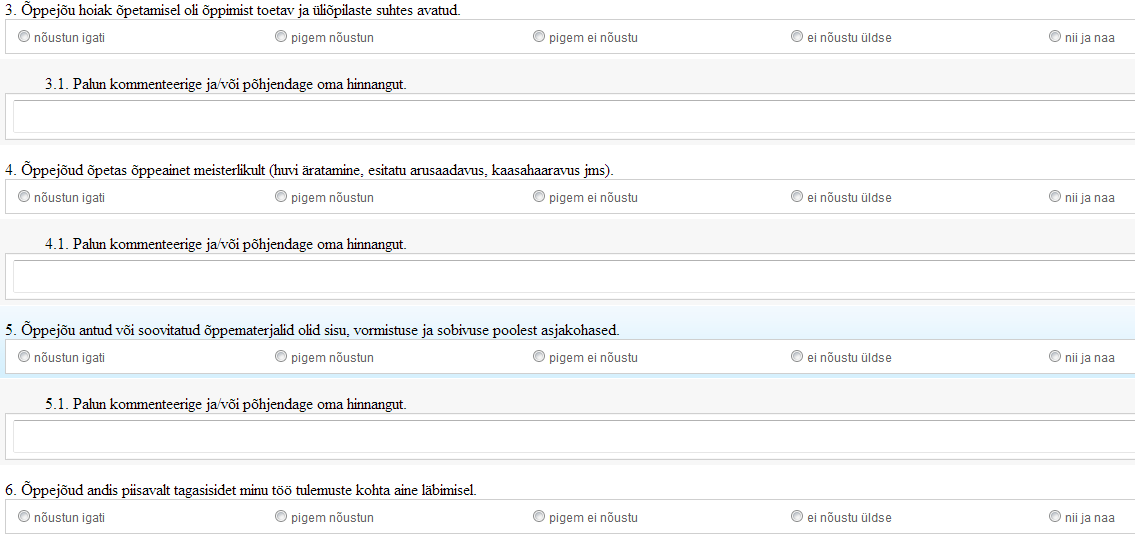
\includegraphics[width=1\textwidth]{ois_tagasiside_toodeldud.png}
\caption{Näide Tartu \"Ulikooli õppeinfo s\"usteemi tagasiside ankeedist, kus rakendatakse Likerti skaalat \cite{UT}}
\label{likert1}
\end{figure}

\begin{figure}[H]
\centering
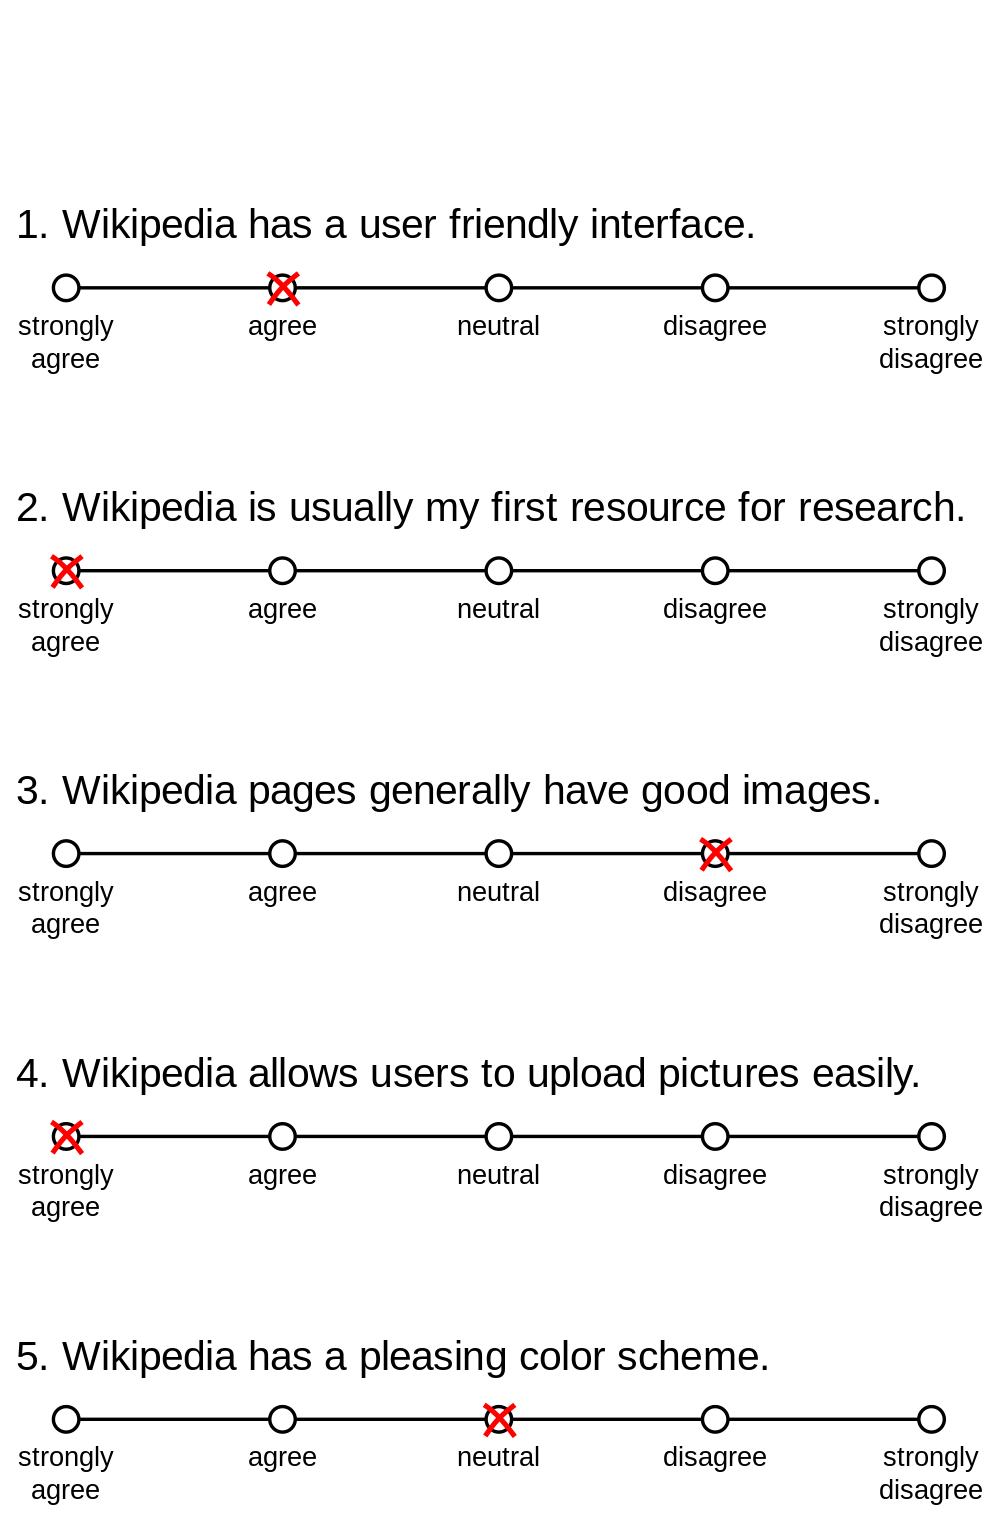
\includegraphics[width=0.85\textwidth]{Example_Likert_Scale.png}
\caption{Näide k\"usimustikust, kus on rakendatud Likerti skaalat; k\"usimused on paigutatud nende järjestikulisuse rõhutamiseks teljele\cite{Smith}}
\label{likert2}
\end{figure}



\subsection{Empiirilised näited}
\label{appendix:empiric}

Järgnevad kovariatsioonimaatriksid on leitud ühe Tartu ülikooli psühholoogide poolt läbiviidud küsimustiku andmete põhjal, jagadas küsimustiku alam\-küsimus\-tikeks. 


\begin{figure}[H]
\begin{small}
\begin{center} 
\begin{tabular} { r r r r r r r r r r r r r }
 \multicolumn{ 12 }{l}{ Kovariatsioonimaatriks} \cr
 \hline 

    3.00  &   1.52  &   1.73  &   1.21  &   0.69  &   1.40  &  -0.53  &  -0.64  &  -0.75  &  -0.56  &  -0.57  &  -0.83 \cr 
      1.52  &   3.25  &   1.37  &   0.70  &   0.78  &   1.01  &  -0.31  &  -0.21  &  -0.17  &  -0.39  &  -0.29  &  -0.65 \cr 
      1.73  &   1.37  &   3.25  &   1.43  &   0.85  &   1.62  &  -0.71  &  -0.77  &  -0.94  &  -0.98  &  -0.65  &  -1.20 \cr 
     1.21  &   0.70  &   1.43  &   2.79  &   0.16  &   1.00  &  -1.03  &  -1.23  &  -0.98  &  -0.87  &  -0.82  &  -0.85 \cr 
     0.69  &   0.78  &   0.85  &   0.16  &   2.67  &   0.82  &  -0.11  &   0.20  &  -0.10  &   0.10  &   0.40  &  -0.09 \cr 
      1.40  &   1.01  &   1.62  &   1.00  &   0.82  &   2.37  &  -0.52  &  -0.48  &  -0.84  &  -0.55  &  -0.37  &  -0.73 \cr 
     -0.53  &  -0.31  &  -0.71  &  -1.03  &  -0.11  &  -0.52  &   1.59  &   1.25  &   0.52  &   0.87  &   0.65  &   0.93 \cr 
     -0.64  &  -0.21  &  -0.77  &  -1.23  &   0.20  &  -0.48  &   1.25  &   2.38  &   0.77  &   1.12  &   0.92  &   1.02 \cr 
     -0.75  &  -0.17  &  -0.94  &  -0.98  &  -0.10  &  -0.84  &   0.52  &   0.77  &   2.30  &   0.81  &   0.75  &   0.68 \cr 
     -0.56  &  -0.39  &  -0.98  &  -0.87  &   0.10  &  -0.55  &   0.87  &   1.12  &   0.81  &   2.14  &   1.00  &   1.25 \cr 
     -0.57  &  -0.29  &  -0.65  &  -0.82  &   0.40  &  -0.37  &   0.65  &   0.92  &   0.75  &   1.00  &   2.09  &   0.69 \cr 
     -0.83  &  -0.65  &  -1.20  &  -0.85  &  -0.09  &  -0.73  &   0.93  &   1.02  &   0.68  &   1.25  &   0.69  &   2.03 \cr 
 \hline 
\end{tabular}


\vspace{10pt}



\begin{tabular}{l | r r r r r}
\hline
 Hinnang & $\lambda_1$ & $\lambda_2$ & $\lambda_3$ & $\lambda_4$ & $glb$ \cr
 Väärtus & 0.39 & 0.60 & 0.43 & 0.73 & 0.77 \cr 
 \hline
 \end{tabular}
 \end{center}
 \end{small}
 \caption{Kahe erineva kuue küsimusega alamküsimustiku kombineerimisel saadud kovariatsioonimaatriks koos reliaabluse hinnangutega  }
  \label{emp:first}
\end{figure} 





\begin{figure}[H]
\begin{small} 
\begin{center}
\begin{tabular} { r r r r r r r r r r r r r }
 \multicolumn{ 12 }{l}{ Kovariatsioonimaatriks } \cr 
 \hline Variable  &   1  &  2  &  3  &  4  &  5  &  6  &  7  &  8  &  9  &  10  &  11  &  12 \cr 
  \hline 
  &  3.00  &  1.52  &  1.73  &  1.21  &  0.69  &  1.40  &  1.39  &  0.90  &  1.27  &  1.15  &  0.58  &  0.83 \cr 
   &  1.52  &  3.25  &  1.37  &  0.70  &  0.78  &  1.01  &  1.10  &  1.73  &  0.94  &  0.85  &  0.56  &  0.70 \cr 
   &  1.73  &  1.37  &  3.25  &  1.43  &  0.85  &  1.62  &  1.19  &  0.61  &  1.85  &  1.28  &  0.61  &  0.85 \cr 
   &  1.21  &  0.70  &  1.43  &  2.79  &  0.16  &  1.00  &  0.64  &  0.26  &  0.93  &  1.49  &  0.14  &  0.53 \cr 
   &  0.69  &  0.78  &  0.85  &  0.16  &  2.67  &  0.82  &  0.77  &  0.99  &  0.64  &  0.10  &  1.61  &  0.56 \cr 
   &  1.40  &  1.01  &  1.62  &  1.00  &  0.82  &  2.37  &  0.98  &  0.74  &  1.17  &  1.02  &  0.74  &  0.90 \cr 
   &  1.39  &  1.10  &  1.19  &  0.64  &  0.77  &  0.98  &  2.39  &  1.26  &  1.12  &  0.66  &  0.61  &  0.72 \cr 
   &  0.90  &  1.73  &  0.61  &  0.26  &  0.99  &  0.74  &  1.26  &  2.91  &  0.55  &  0.43  &  0.82  &  0.77 \cr 
   &  1.27  &  0.94  &  1.85  &  0.93  &  0.64  &  1.17  &  1.12  &  0.55  &  2.52  &  0.81  &  0.45  &  0.80 \cr 
   &  1.15  &  0.85  &  1.28  &  1.49  &  0.10  &  1.02  &  0.66  &  0.43  &  0.81  &  2.19  &  0.25  &  0.55 \cr 
   &  0.58  &  0.56  &  0.61  &  0.14  &  1.61  &  0.74  &  0.61  &  0.82  &  0.45  &  0.25  &  2.43  &  0.54 \cr 
   &  0.83  &  0.70  &  0.85  &  0.53  &  0.56  &  0.90  &  0.72  &  0.77  &  0.80  &  0.55  &  0.54  &  1.35 \cr 
 \hline 
\end{tabular}


\vspace{10pt}



\begin{tabular}{l | r r r r r}
\hline
 Hinnang & $\lambda_1$ & $\lambda_2$ & $\lambda_3$ & $\lambda_4$ & $glb$ \cr
 Väärtus & 0.79 & 0.87 & 0.86 & 0.93 & 0.93 \cr 
 \hline
 \end{tabular}
 \end{center}
 \end{small}

 \caption{Kahe sama konstruktsiooni mõõtva kuue küsimusega alamküsimustike kombineerimisel saadud kovariatsioonimaatriks koos reliaabluse hinnangutega  }
  \label{emp:second}
\end{figure} 



\begin{figure}[H]
\begin{small} 
\begin{center}
\begin{tabular} { r r r r r r r r r r r r r }
 \multicolumn{ 12 }{l}{Kovariatsioonimaatriks} \cr 

  \hline 
    1.99  &   0.39  &   0.37  &   0.98  &   0.85  &   0.70  &  -0.48  &  -0.49  &  -0.39  &  -0.43  &  -0.25  &  -0.27 \cr 
     0.39  &   2.15  &   0.38  &   0.79  &   0.50  &   0.28  &  -0.60  &  -0.39  &  -0.27  &  -0.05  &  -0.19  &  -0.05 \cr 
     0.37  &   0.38  &   2.12  &   0.45  &   0.74  &   0.70  &  -0.41  &  -0.10  &  -0.06  &   0.06  &  -0.02  &   0.07 \cr 
     0.98  &   0.79  &   0.45  &   3.06  &   0.95  &   0.34  &  -0.59  &  -0.64  &  -0.36  &  -0.14  &  -0.04  &   0.05 \cr 
     0.85  &   0.50  &   0.74  &   0.95  &   2.90  &   0.77  &  -0.32  &  -0.58  &  -0.05  &   0.05  &   0.22  &   0.32 \cr 
     0.70  &   0.28  &   0.70  &   0.34  &   0.77  &   2.65  &  -0.47  &  -0.45  &  -0.45  &  -0.37  &  -0.39  &  -0.38 \cr 
    -0.48  &  -0.60  &  -0.41  &  -0.59  &  -0.32  &  -0.47  &   1.99  &   0.58  &   0.51  &   0.38  &   0.31  &   0.47 \cr 
    -0.49  &  -0.39  &  -0.10  &  -0.64  &  -0.58  &  -0.45  &   0.58  &   1.86  &   0.59  &   0.30  &   0.03  &   0.31 \cr 
    -0.39  &  -0.27  &  -0.06  &  -0.36  &  -0.05  &  -0.45  &   0.51  &   0.59  &   1.63  &   0.63  &   0.45  &   0.81 \cr 
    -0.43  &  -0.05  &   0.06  &  -0.14  &   0.05  &  -0.37  &   0.38  &   0.30  &   0.63  &   1.41  &   0.63  &   1.01 \cr 
    -0.25  &  -0.19  &  -0.02  &  -0.04  &   0.22  &  -0.39  &   0.31  &   0.03  &   0.45  &   0.63  &   1.79  &   1.11 \cr 
    -0.27  &  -0.05  &   0.07  &   0.05  &   0.32  &  -0.38  &   0.47  &   0.31  &   0.81  &   1.01  &   1.11  &   2.33 \cr 
 \hline 
\end{tabular}


\vspace{10pt}



\begin{tabular}{l | r r r r r}
\hline
 Hinnang & $\lambda_1$ & $\lambda_2$ & $\lambda_3$ & $\lambda_4$ & $glb$ \cr
 Väärtus & 0.39 & 0.53 & 0.43 & 0.68 & 0.70 \cr 
 \hline
 \end{tabular}
 \end{center}
 \end{small}

 \caption{Kahe erineva kuue küsimusega alamküsimustiku kombineerimisel saadud kovariatsioonimaatriks koos reliaabluse hinnangutega  }  
  \label{emp:third}
\end{figure} 






\subsection{Programmiteegi implementatsioon}
\label{appendix:code}


\begin{customFloatWrap}
\begin{minted}[bgcolor=background_example, tabsize=2, fontsize=\footnotesize , linenos=true, numberblanklines=false]{python}


def calculate_lambda_1(cov_matrix):
    u""" 
    Based on Guttman,1945, for calculations using Jackson,
    Aguvwamba,1977,[569].
    """
    n = check_that_matrix_is_square_and_fix_n(cov_matrix)
    def sum_of_main_diagonal():
        summ = 0
        for i in xrange(n):
            summ += cov_matrix[i,i]
        return summ

    return 1 - (sum_of_main_diagonal()/
    	calculate_sum_of_covariance_matrix_elements(cov_matrix, n))

\end{minted}
\captionof{Programm}{Funktsioon hinnangu $\lambda_1$ leidmiseks}
\end{customFloatWrap}

\vspace{10pt}


\begin{customFloatWrap}
\begin{minted}[bgcolor=background_example, tabsize=2, fontsize=\footnotesize ,  linenos=true, numberblanklines=false]{python}
def calculate_lambda_2(cov_matrix):
    u"""
    Using Guttman,1945,[259] definition.
    """
    def sum_of_squares_of_non_diagonal_matrix_elements():
        summ = 0
        for i in xrange(n):
            for j in xrange(i):
                    summ += cov_matrix[i,j]**2 
        return 2*summ
    
    n = len(cov_matrix)
    l1 = calculate_lambda_1(cov_matrix)
    sum_of_squares = sum_of_squares_of_non_diagonal_matrix_elements()
    under_square_root =((n)/(n-1)* sum_of_squares)**(1/2)
    return l1 + (under_square_root/
        calculate_sum_of_covariance_matrix_elements(cov_matrix))
\end{minted}
\captionof{Programm}{Funktsioon hinnangu $\lambda_2$ leidmiseks}
\end{customFloatWrap}


\vspace{10pt}

\begin{customFloatWrap}
\begin{minted}[bgcolor=background_example, tabsize=2, fontsize=\footnotesize ,  linenos=true, numberblanklines=false]{python}
def calculate_lambda_3(cov_matrix):
    number_of_items = len(cov_matrix)
    return (number_of_items/(number_of_items-1))*calculate_lambda_1(cov_matrix)      
  
\end{minted}
\captionof{Programm}{Funktsioon hinnangu $\lambda_3$ leidmiseks}
\end{customFloatWrap}

\vspace{10pt}
        
\begin{customFloatWrap}
\begin{minted}[bgcolor=background_example, tabsize=2, fontsize=\footnotesize , linenos=true, numberblanklines=false]{python}

import numpy as np

def calculate_lambda_4(cov_matrix):
    u"""
    Lambda 4, based on Guttman, 1945, using the implementation of Jackson,
    Agunwamba, 1977.
    Based on idea that we try to best possible split (u is a vector,
     with elements either 1 or -1, ones will be in one split, 
     minus ones in another) .
    NAIVE IMPLEMENTATION, works with relativiely low N, 
    better approches available,  see Benton, 2013.
    """
    
    def objective_function(u):
        return u.T.dot(cov_matrix.dot(u))

    
    def try_vectors():
        u"""
        Idea : generate half of all possible vectors of length n,
         such that if vector v is in, vector -v is not. 
        Using binary representation as string,
         from 2**(n-1) to 2**n, coding "0" to "-1"
        """
        smallest = np.Infinity
        result_vector = []
        l = []
        for i in xrange(2**(n-1),2**n):
            binary_of_i = np.binary_repr(i,width=n)
            binary_of_i_int = [ 1 if x == u"1" else -1 for x in binary_of_i]
            u = np.array(binary_of_i_int)
            result = objective_function(u)
            if result < smallest:
                smallest = result
                result_vector = u
        return smallest
             
    def calc_lambda(smallest):
        return 1 - (smallest/
            util.calculate_sum_of_covariance_matrix_elements(cov_matrix, n))
        
    n = util.check_that_matrix_is_square_and_fix_n(cov_matrix)
    return calc_lambda(try_vectors())

\end{minted}
\captionof{Programm}{Funktsioon hinnangu $\lambda_4$ leidmiseks}
\end{customFloatWrap}

\vspace{10pt}

\begin{customFloatWrap}
\begin{minted}[bgcolor=background_example, tabsize=2, fontsize=\footnotesize , linenos=true, numberblanklines=false]{python}

import cvxpy as cv
import numpy as np

u""""
Idea: Observed covariance matrix  is of observed scores. 
That matrix is sum of true score coviarance matrix and error covariance matrix.
As errors don't correlate with anything else than themselves,
 the last is diagonal matrix. So, C_obs = C_true + C_error
We look to maximize error (to find the worst possible case), 
that is the same as minimizing the trace of C_true.
More can be found in Jackson,Agunwamba,1977 and Woodhouse,Jakson, 1977.
"""

class Glb(object):
    def __init__(self,cov_matrix):
        self._cov_matrix = cov_matrix
        self._constraints = []
        self._n = util.check_that_matrix_is_square_and_fix_n(cov_matrix)
        self._cov_matrix = np.matrix(cov_matrix)
        self._generate_matrix_variables()
        self._divide_covariance_matrix_of_into_error_and_true_score()
        self._fix_error_cov_matrix_diagonal_fields_constraints()
        self._error_cov_matrix_non_diagonal_fields_are_0()
        self._prepare_program()
        self._solve_program()
        self._answer = self._calculate_Glb()

    def _generate_matrix_variables(self):
        self._true_cov_matrix = cv.semidefinite(self._n,
             name=u"true_cov_matrix")
        self._error_cov_matrix = cv.Variable(self._n, self._n, 
            name=u"error_cov_matrix") 
    
    
    def _divide_covariance_matrix_of_into_error_and_true_score(self):
        u"""
        Constraint that C_obs = C_true + C_error
        """
        self._constraints.append(self._error_cov_matrix+
            self._true_cov_matrix == self._cov_matrix)
        
    def _fix_error_cov_matrix_diagonal_fields_constraints(self):
        u"""
        Error covariance matrix must be semidefinite,
         meaning that all elements on the diagonal must be positive.
        """
        for i in xrange(self._n):
            self._constraints.append(self._error_cov_matrix[i,i] >= 0)

    def _error_cov_matrix_non_diagonal_fields_are_0(self):
        u"""
        Covariance between different errors is 0
        """
        for i in xrange(self._n):
            for j in xrange(self._n):
                if (i != j):
                    self._constraints.append(
                        self._error_cov_matrix[i,j] == 0) 

        
    def _prepare_program(self):
        u"""
        Minimize trace of true score covirance matrix
        """
        self._p = cv.Problem(cv.Minimize(
            sum([self._true_cov_matrix[i,i] for i in xrange(self._n)])),
            self._constraints)
        if not self._p.is_dcp():
            raise Exception(u"Non-DCP glb, something went terrible wrong")
            
            
    def _solve_program(self):

        try:
            self._p.solve()
        except:
            raise Exception(u"Program was unable to find glb")
        
    
    def _calculate_Glb(self):
        return 1 - (sum(
        	[self._error_cov_matrix.value[i,i] for i in xrange(self._n)])/
            util.calculate_sum_of_covariance_matrix_elements(
                self._cov_matrix,self._n)
        

    def get_answer(self):
        return self._answer
        
\end{minted}
\captionof{Programm}{Klass hinnangu $glb$ leidmiseks}
\end{customFloatWrap}

\vspace{10pt}

\begin{customFloatWrap}
\begin{minted}[bgcolor=background_example, tabsize=2, fontsize=\footnotesize]{python}

def check_that_matrix_is_square_and_fix_n(input_matrix):      
    def check_that_matrix_is_square():   
        for row in input_matrix:
            if len(row) != n:
                raise Exception(u"Matrix not square or missing data")  
    n = len(input_matrix) 
    check_that_matrix_is_square()
    return n

def fix_number_of_rows(input_matrix):
    def check_that_matrix_is_complete():   
        for row in input_matrix:
            if len(row) != n:
                raise Exception(u"Matrix not square or missing data")
    n = len(input_matrix[0])
    check_that_matrix_is_complete()
    return n
    

def calculate_sum_of_covariance_matrix_elements(cov_matrix,n = None):
    if n == None:
        n = check_that_matrix_is_square_and_fix_n(cov_matrix)
    summ = 0
    for i in xrange(n):
        for j in xrange(n):
            summ += cov_matrix[i,j]
    return summ

\end{minted}
\captionof{Programm}{Eelnevates programmides kasutatud abifunktsioonid}
\end{customFloatWrap}


\pagebreak 

\makeatletter
\newpage
\pagestyle{empty}
\thispagestyle{empty}

\subsection{Litsents}


\textbf{Lihtlitsents lõputöö reprodutseerimiseks ja
lõputöö üldsusele kätte\-saa\-davaks tegemiseks.}


Mina, \@author\ (sünnikuupäev: 11.11.1988)
\begin{enumerate}
\item annan Tartu Ülikoolile tasuta loa (lihtlitsentsi)
enda loodud teose
\begin{center}
\@title,
\end{center}
mille juhendaja on Margus Niitsoo,
\begin{enumerate}
\item reprodutseerimiseks säilitamise ja üldsusele
kättesaadavaks tegemise eesmärgil, sealhulgas
digitaalarhiivi DSpace'i lisamise eesmärgil kuni
autoriõiguse kehtivuse tähtaja lõppemiseni;
\item üldsusele kättesaadavaks tegemiseks Tartu Ülikooli
veebikeskkonna kaudu, sealhulgas digitaalarhiivi
DSpace'i kaudu kuni autoriõiguse kehti\-vuse tähtaja lõppemiseni.
\end{enumerate}
\item olen teadlik, et punktis 1 nimetatud õigused jäävad
alles ka autorile.
\item kinnitan, et lihtlitsentsi andmisega ei rikuta teiste
isikute intellektuaal\-omandi ega isikuandmete kaitse
seadusest tulenevaid õigusi.
\end{enumerate}

\vfill

\begin{center}
Tartu,  \today
\end{center}

\makeatother


\end{subappendices}
\end{document}
